\documentclass{article}
\usepackage[utf8]{inputenc}

\title{Multivariable Calculus}
\author{Josh Joseph}
\date{Summer 2020}

\addtolength{\oddsidemargin}{-.875in}
\addtolength{\evensidemargin}{-.875in}
\addtolength{\textwidth}{1.75in}
\addtolength{\topmargin}{-.875in}
\addtolength{\textheight}{1.75in}

\usepackage{amsmath}
\usepackage{amssymb}
\usepackage{gensymb}
\usepackage{graphicx}
\usepackage{float}
\usepackage{amsthm}
\usepackage{amsbsy}
\usepackage{etoolbox}
\usepackage{esvect}

\AtBeginEnvironment{gather}{\setcounter{equation}{0}}

\renewcommand{\qedsymbol}{$\blacksquare$}
\let\oldvec\vv
\renewcommand{\vv}[1]{\oldvec{\mathbf{#1}}}
\let\oldhat\hat
\renewcommand{\hat}[1]{\oldhat{\mathbf{#1}}}
\let\vl\langle
\let\vr\rangle
\let\ve\hat
\renewcommand{\ve}[1]{\vl#1\vr}
\let\d\hat
\renewcommand{\d}{\hspace{3pt}\textrm{d}}

\makeatletter
\newcommand*\vdot{\mathpalette\vdot@{.5}}
\newcommand*\vdot@[2]{\mathbin{\vcenter{\hbox{\scalebox{#2}{$\m@th#1\bullet$}}}}}
\makeatother

\begin{document}

\maketitle

\tableofcontents
\newpage
\setcounter{section}{10}
\section{Parametric Equations and Polar Coordinates}

\subsection{Curves Defined By Parametric Equations}
\textrm{}
Some curves cannot be defined in the form of $y=f(x)$ since they fail the vertical line test.

Instead, a curve can be defined(in this case with 2D space) with one or more \textbf{parametric equations}, where $x$ and $y$ are given as functions of a parameter $t$.
\begin{gather*}
    x=f(t)\\
    y=g(t)
\end{gather*}

As $t$ varies, the points $(f(t),g(t))$ trace out a \textbf{parametric curve}. Consecutive points on this curve are at equal time intervals, but not necessarily equal distances.

An arrowhead can be used to specify the direction of time on such a curve. The domain can also be restricted as shown below:
\begin{gather*}
    x=f(t)\\
    y=g(t)\\
    a \leqslant t \leqslant b
\end{gather*}
In this case, the traced curve would be drawn from \textbf{initial point} $(f(a),g(a))$ to \textbf{terminal point} $(f(b),g(b))$

For example, the curve given by the set of parametric equations $x=cos(t)$ and $y=sin(t)$ would trace out a circle as seen in Fig. \ref{unitcirc}. \\
\begin{figure}[H]
\begin{center}
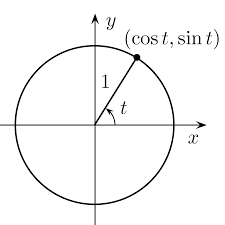
\includegraphics[scale=0.5]{UnitCircle.png}
\caption{The Unit Circle and Parametric Equations}
\label{unitcirc}
\end{center}
\end{figure}

Since these curves are defined as a function of a parameter, multiple different equations can describe the same curve. For example, $x=cos(2t)$ and $y=sin(2t)$. Because the range of the $sin$ and $cos$ functions are the same, these equations would draw out the same curve as Figure \ref{unitcirc}.

A \textbf{family} of parametric equations is a group of equations with the same parameter that trace out similar curves, normally by changing a constant. Circles, Lines, and Cycloids can be traced out using families of parametric equations.

\subsection{Calculus with Parametric Curves}
\subsubsection{Slope of a Parametric Curve}
By eliminating the parameter $t$ the parametric equations $x=f(t)$ and $y=g(t)$ can be written in the general form $h(x)$:
\begin{gather*}
    y = g(t) = h(f(t))
\end{gather*}
Applying the chain rule,
\begin{gather*}
y'(t) = g'(t) = h'(f(t))*f'(t) = h'(x)*f'(t)
\end{gather*}
If $f'(t) \neq 0$ then
\begin{gather*}
    h'(x) = \frac{g'(t)}{f'(t)}
\end{gather*}
This can be rewritten as:
\begin{gather*}
    \frac{d}{dx} (y) = \frac{dy}{dx} = \frac{\frac{dy}{dt}}{\frac{dx}{dt}}
\end{gather*}
By replacing $y$ with $\frac{dy}{dx}$:
\begin{gather*}
    \frac{d}{dx} (\frac{dy}{dx}) = \frac{d^2y}{dx^2} = \frac{\frac{d}{dt} (\frac{dy}{dx})}{\frac{dx}{dt}}
\end{gather*}
\subsubsection{Areas and Volumes with Parametrics}
Since the area under a curve of $y = h(x)$ is given by $\int_a^b h(x) dx$, a similar formula can be obtained for parametric equations where $x=f(t)$ and $y=g(t)$:
\begin{gather*}
    Area = \int_a^b y\hspace{2pt}dx = \int_c^d y \hspace{2pt} \frac{dx}{dt} \hspace{2pt}dt = \int_c^d g(t) * f'(t) \hspace{2pt} dt
\end{gather*}
Where $c$ is the left endpoint and $d$ is the right endpoint.
\linebreak\linebreak
A similar formula can be proved for the arc length of a parametric curve:
\begin{gather*}
    Arc\hspace{2pt}Length = \int_a^b \sqrt{1+(\frac{dy}{dx})^2} \hspace{3pt}dx
    = \int_c^d \sqrt{1+(\frac{\frac{dy}{dt}}{\frac{dx}{dt}})^2} \hspace{3pt} \frac{dx}{dt} \hspace{2pt} dt
    \linebreak\linebreak
    = \int_c^d \sqrt{(\frac{dx}{dt})^2 + (\frac{dy}{dt})^2} \hspace{3pt} dt
\end{gather*}
Even if the parametric curve cannot be expressed in the form $y=h(x)$ a limit Riemann sum can be used to prove this equation true.

The Surface Area of a solid of revolution can be derived similarly, using the non-parametric formula.

\begin{gather*}
    SA = \int_c^d 2\pi y \sqrt{(\frac{dx}{dt})^2 + (\frac{dy}{dt})^2} \hspace{3pt} dt
\end{gather*}
\subsection{Polar Coordinates}
\subsubsection{Defining Polar Coordinates}
Sometimes Cartesian coordinates are not convenient to represent some functions, where \textbf{polar coordinates} could be used. A \textbf{polar axis}, corresponding to the x-axis in Cartesian, is used as the base axis. Every point $P$ in the plane can be represented with two coordinates $(r,\theta)$, where $r$ is the distance from the origin to $P$ and $\theta$ is the angle between the polar axis and the line drawn from the origin to $P$, as seen in Figure \ref{polar}.

A point $(-r,\theta)$ can be defined as $(r,\theta+\pi)$. Because points are specified using angles around the polar axis, multiple coordinates can specify the same location. For example, the coordinates $(r,\theta)$ can also be written as:
\begin{gather*}
(r, \theta+2\pi n)
\end{gather*}
\begin{center}
    or
\end{center}
\begin{gather*}
(-r, \theta+(2n+1)\pi)
\end{gather*}
\begin{figure}[H]
\begin{center}
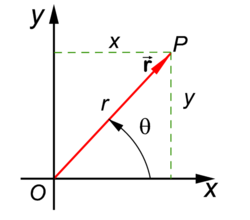
\includegraphics[scale=5]{MC11-polar.png}
\caption{Polar Coordinates}
\label{polar}
\end{center}
\end{figure}
Converting from polar to Cartesian coordinates can be done using trigonometric functions of $\theta$.
\begin{gather*}
    x = r cos(\theta)\hspace{50pt} y = r sin(\theta)
\end{gather*}
To convert from Cartesian to polar use:
\begin{gather*}
    r^2 = x^2 + y^2 \hspace{50pt} tan\hspace{2pt}\theta = \frac{y}{x}
\end{gather*}
The graph of a polar equation involves all points that can be represented using $(r,\theta)$ and whose coordinates make the equation true.\\
\subsubsection{Symmetry}
Polar symmetry can be used to help graph polar equations easier. Similar to Cartesian symmetry in $x$ and $y$, there are a few rules for polar symmetry.\\

If the Polar equation is unchanged when:
\begin{enumerate}
    \item $\theta$ is switched with $-\theta$, then the graph is symmetric over the polar axis.
    \item $r$ is switched with $-r$ or $\theta$ is replaced with $\theta + \pi$, the curve is symmetric about the origin(180 degree rotation symmetry).
    \item $\theta$ is replaced by $\pi - \theta$, then the graph is symmetric about the '$y$' axis, (the line $\theta = \frac{\pi}{2}$).
\end{enumerate}
\subsubsection{Slope of a Polar Curve}
To find the instantaneous slope or tangent line at a point on a polar curve, rewrite the polar function $r=f(\theta)$ as parametric equations with $\theta$ as a parameter.
\begin{gather*}
    x = r cos(\theta) = f(\theta)cos(\theta)\hspace{20pt}y = r sin(\theta) = f(\theta)sin(\theta)
\end{gather*}
Now by finding the slope of the now-parametric curve:
\begin{gather*}
    \frac{dy}{dx} = \frac{\frac{dy}{d\theta}}{\frac{dx}{d\theta}}
    = \frac{\frac{dr}{d\theta}*sin(\theta) + r cos(\theta)}{\frac{dr}{d\theta}*cos(\theta) - rsin(\theta)}
\end{gather*}
For the special case $r=0$:
\begin{gather*}
    \frac{dy}{dx} = tan(\theta) \hspace{5pt} for \hspace{5pt} \frac{dr}{d\theta} \neq 0
\end{gather*}
\subsection{Areas and Lengths in Polar Coordinates}
\subsubsection{Areas in Polar}
The area of a region bounded by a polar equation can be derived from the area of a sector of a circle(since polar equations also depend on the angle):
\begin{gather*}
    A = \frac{1}{2}r^2\theta
\end{gather*}
Where $A$ is the area and $\theta$ is measured in radians.

Given a region bounded by a curve $r=f(\theta)$ and the lines given by the polar equations $\theta=c$ and $\theta=d$, $0 < d - c \leqslant 2\pi$. Dividing the region into areas with equal width $\Delta \theta$, the area of Region $i$ can be approximated as:
\begin{gather*}
    A_i \approx \frac{1}{2} [f(\theta_i)]^2 * \Delta \theta
\end{gather*}
And so, a Riemann sum can be used to improve the approximation as $\Delta \theta \to 0$ and $n \to \infty$.
\begin{gather*}
    A = \lim_{n \to \infty} \sum_{i=1}^{n} \frac{1}{2} [f(\theta_i)]^2 * \Delta \theta = \int_c^d \frac{1}{2} [f(\theta_i)]^2 \hspace{2pt}d\theta
\end{gather*}
Since $r=f(\theta)$, this can also be written in a form similar to the circle sector formula:
\begin{gather*}
    A = \int_c^d \frac{1}{2} r^2 \hspace{2pt}d\theta
\end{gather*}
The area between two polar curves $f(\theta)$ and $g(\theta)$ can be derived using integral rules, where $j$ and $k$ are the angle coordinate of the points of intersection on both curves:
\begin{gather*}
    A = \frac{1}{2} \int_j^k ([f(\theta)]^2 - [g(\theta)]^2) \hspace{2pt}d\theta
\end{gather*}
The above works for $f(\theta) \geqslant g(\theta) \geqslant 0$ for all $\theta$ between $j$ and $k$.
\subsubsection{Lengths in Polar}
The Arc Length of a polar curve $r=f(\theta)$ between $\theta = a$ and $\theta = b$ can be found by treating $\theta$ as a parameter. This means that the parametric equations describing these are:

\begin{gather*}
    x = r * cos(\theta) = f(\theta)*cos(\theta)
\\
    y = r * sin(\theta) = f(\theta) * sin(\theta)
\end{gather*}
Using the product rule, where $r' = \frac{dr}{d\theta}$:
\begin{gather*}
    \frac{dx}{d\theta} = r' * cos(\theta) - r * sin(\theta)
    \\
    \frac{dy}{d\theta} = r' * sin(\theta) + r * sin(\theta)
\end{gather*}
Squaring both and adding yields:
\begin{gather*}
    (\frac{dx}{d\theta})^2 + (\frac{dy}{d\theta})^2 = (r')^2(sin^2(\theta) + cos^2(\theta)) + r^2(sin^2(\theta) + cos^2(\theta)) = r^2 + (\frac{dr}{d\theta})^2
\end{gather*}
Using the arc length formula(see 11.2), with $\theta$ as a parameter:
\begin{gather*}
    Arc\hspace{2pt}Length = \int_a^b \sqrt{r^2 + (\frac{dr}{d\theta})^2} \hspace{2pt} d\theta
\end{gather*}
\subsection{Conic Sections}
Parabolas, ellipses, and hyperbolas can be formed by the intersection of a plane with a cone, which is why they are often called \textbf{conics} or \textbf{conic sections}.
\subsubsection{Parabolas}
A \textbf{parabola} is formed when a plane cuts into a cone at an angle so that it intersects the cone's base. It is the set of points that are equidistant from a \textbf{focus} point $F$ and a line(called the \textbf{directrix}.) The point directly halfway between the directrix and focus lies on the parabola, and this is the \textbf{vertex}. The perpendicular through $F$ and intersecting the directrix is the parabola's \textbf{axis}.

If the focus is on the origin, then the focus of a basic parabola can be defined as the point $(0,p)$ and the directrix $y=-p$.

Using the distance formula, the distance between any point $P(x,y)$ on the parabola to the focus is:
\begin{gather*}
    |PF| = \sqrt{x^2 + (y-p)^2}
\end{gather*}
Similarly, the distance from the line to $P$(perpendicularly) is:
\begin{gather*}
    d(P,directrix) = |y+p|
\end{gather*}
By definiton, these two should be equal.
\begin{gather*}
    \sqrt{x^2 + (y-p)^2} = |y+p|\\
    x^2 + (y-p)^2 = (y+p)^2\\
    x^2 + y^2 -2py + p^2 = y^2 + 2py + p^2\\
    x^2 = 4py
\end{gather*}
If $a = \frac{1}{4p}$, then the standard form of a parabola based on the origin is:
\begin{gather*}
    y = \frac{x^2}{4p}\\
    y = ax^2
\end{gather*}
If $p > 0$ then the parabola opens up, and the opposite when $p < 0$. Replacing $y$ and $x$ reflects the parabola over the line $y=x$:
\begin{gather*}
    y^2 = 4px
\end{gather*}
\subsubsection{Ellipses}
An \textbf{ellipse} is formed when a plane intersects a cone and comes out on the other side without touching the base. It is the set of all points in a plane such that the sum of the distances from two focal points(\textbf{foci}) is constant.

Assuming the simplest case, where the foci are located on the x-axis at equal distances from the origin, the foci are located at points $(c,0)$ and $(-c,0)$. The constant distance sum is $2a$, greater than zero.

$P(x,y)$  is a point on the ellipse if
\begin{gather*}
    |PF_1| + |PF_2| = 2a\\
    \sqrt{(x+c)^2 + y^2} + \sqrt{(x-c)^2 + y^2} = 2a\\
    \sqrt{(x-c)^2 + y^2} = 2a - \sqrt{(x+c)^2 + y^2}\\
    x^2 - 2xc + c^2 + y^2 = 4a^2 - 4a\sqrt{(x+c)^2 + y^2} + x^2 + 2xc + c^2 + y^2\\
    a\sqrt{(x+c)^2+y^2} = a^2 + cx\\
    a^2(x^2 + 2xc + c^2 + y^2) = a^4 + 2a^2xc + x^2c^2\\
    (a^2 - c^2)x^2 + a^2y^2 = a^2(a^2-c^2)
\end{gather*}
Since $2c < 2a$(Triangle Inequality Theorem), we can define $b^2 = a^2 - c^2 > 0$. This becomes:
\begin{gather*}
    b^2x^2 + a^2y^2 = a^2b^2\\
    \frac{x^2}{a^2} + \frac{y^2}{b^2} = 1
\end{gather*}
When $y = 0$, the x-intercepts of the ellipse are $x = \pm a$. These points $(\pm a,0)$ are the the \textbf{vertices} of the ellipse and lie on its \textbf{major axis}. The y-intercepts are found to be $y = \pm b$. Since $x$ and $y$ are both squared in the equation, the ellipse is symmetric around both axes. A circle is just an ellipse where both foci are at the same point($c = 0$), and $r = a = b$.
\subsubsection{Hyperbolas}
A \textbf{hyperbola} made up of two branches can be formed by cutting two bases of a conic cone with a plane inclined vertically. It is the set of all points in a plane where the differences of distances from two \textbf{foci} are constant. Similar to an ellipse, where the distances from the points are added.

This means that for any point $P(x,y)$ on the hyperbola, $|PF_1| - |PF_2| = \pm 2a$, where $a$ is a constant. Using a similar method to an ellipse, the equation for any hyperbola is:
\begin{gather*}
    \frac{x^2}{a^2} - \frac{y^2}{b^2} = 1
\end{gather*}
Where the foci are at $x = \pm c$ so that $c^2 = a^2 + b^2$, with vertices at $x = \pm a$. The slant asymptotes are at $y = \pm (\frac{b}{a})x$. If the ellipse's major axis is on or parallel to the y-axis:
\begin{gather*}
    \frac{y^2}{a^2} - \frac{x^2}{b^2} = 1
\end{gather*}
Where the foci are at $y = \pm c$ so that $c^2 = a^2 + b^2$, with vertices at $y = \pm a$. The slant asymptotes are at $y = \pm (\frac{a}{b})x$.
\subsubsection{Shifting Conics}
The above equations were derived for a conic with major axis on the x-axis. These conics can be shifted by replacing $x$ and $y$ with $(x-h)$ and $(y-k)$ where $h$ and $k$ are the horizontal and vertical shifts.
\subsection{Conics in Polar Coordinates}
Instead of defining the ellipse and hyperbola with just foci, a more uniform definition can be applied to all conics:

Let point $F$ be a focus and $l$ be a directrix. $e$ is a constant, the \textbf{eccentricity}. A conic can be defined as the set of all points $P$ in a plane where
\begin{gather*}
    \frac{|PF|}{|Pl|} = e
\end{gather*}
This conic is an ellipse if $e < 1$, a parabola if $e = 1$, and a hyperbola if $e > 1$.
\begin{proof}
If $e = 1$, then the above becomes the definition of a parabola.
\\By converting $P$ to polar coordinates$(r,\theta)$, and setting $F$ at the origin:
\begin{gather*}
    |PF| = r \hspace{5pt} |Pl| = d - x = d - r cos(\theta)
\end{gather*}
Since $|PF| = e|Pl|$,
\begin{gather*}
    r = e(d - r cos(\theta))
\end{gather*}
Squaring both sides, and using $r^2 = x^2 + y^2$:
\begin{gather*}
    (1-e^2)x^2 + 2de^2x + y^2 = e^2d^2\\
    (x+\frac{e^2d}{1-e^2})^2 + \frac{y^2}{1-e^2} = \frac{e^2d^2}{(1-e^2)^2}
\end{gather*}
By completing the square above, that resembles the equation of an ellipse for $e < 1$ since $1-e^2 \geqslant 0$.
\begin{gather*}
    \frac{(x-h)^2}{a^2} + \frac{y^2}{b^2} = 1\\
    h = \frac{-e^2d}{1-e^2}\hspace{25pt}a^2 = \frac{e^2d^2}{(1-e^2)^2}\hspace{25pt}b^2 = \frac{e^2d^2}{1-e^2}
\end{gather*}
Finding the foci of this ellipse comes down to this,
\begin{gather*}
    c^2 = a^2 - b^2 = \frac{e^4d^2}{(1-e^2)^2}\\
    c = \frac{e^2d}{1-e^2} = -h
\end{gather*}
Remember the foci are at $(\pm c, 0)$. Now reducing two of the above equations yields,
\begin{gather*}
    e^2 = \frac{c^2}{a^2}\\
    e = \frac{c}{a}
\end{gather*}
If $e > 1$, that means that $1-e^2$ is now negative, which would only change the sign of $b^2$:
\begin{gather*}
    \frac{(x-h)^2}{a^2} - \frac{y^2}{b^2} = 1
\end{gather*}
This now fits the last case, the equation of the hyperbola.
\end{proof}
Since $r = e(d-rcos(\theta)$, the polar form of a conic is:
\begin{gather*}
    r = \frac{ed}{1 + cos(\theta)}
\end{gather*}
Now the directrix could be on the left too, in which case $x = -d$. Or it could be parallel to the y-axis where $y = \pm d$.
\begin{gather*}
    r = \frac{ed}{1 \pm e\hspace{2pt} cos(\theta)} \hspace{5pt}or \hspace{5pt}r = \frac{ed}{1 \pm e\hspace{2pt} sin(\theta)}
\end{gather*}
Which is an ellipse if $e < 1$, a parabola if $e = 1$, or a hyperbola if $e > 1$.
\section{Infinite Sequences and Series}
\subsection{Sequences}
\subsubsection{Defining Sequences}
A \textbf{sequence} is similar to a list of numbers that have an order:
\begin{gather*}
    a_1,a_2,a_3,a_4,...a_n
\end{gather*}
Where $a_1$ is the \textit{first term}, and $a_2$ is the \textit{second term}, so $a_n$ is the \textit{nth term}.

With infinite sequences, the sequence never ends, so every term $a_n$ has a term after it $a_{n+1}$.

Function properties can also be used by defining a function $f(n) = a_n$ where the domain is the positive integers.

A sequence can be defined explicitly($a_n=2n$) or implicitly($a_n = 5 + a_{n-1}$).
\subsubsection{Limits of Sequences}
Some sequences, such as $a_n = \frac{n}{n+1}$, can converge upon a certain value. This is seen by graphing $f(n) = \frac{n}{n+1}$. $a_n$ seems to be approaching 1 as $n$ increases unbounded.
\begin{gather*}
    1 - \frac{n}{n+1} = \frac{n-n+1}{n+1} = \frac{1}{n+1}
\end{gather*}
So by increasing $n \to \infty$:
\begin{gather*}
    \lim_{n\to \infty} \frac{1}{n+1} = 0
\end{gather*}
This means that
\begin{gather*}
    \lim_{n\to \infty} \frac{n}{n+1} = 1
\end{gather*}
Any sequence $\{a_n\}$ with a limit $L$ can be written as
\begin{gather*}
    \lim_{n\to \infty} a_n = L
\end{gather*}
This is true if $a_n$ can get arbitrarily close to $L$ by choosing some applicable(usually large) value of $n$. If $\lim_{n\to \infty} a_n$ exists, then $a_n$ \textbf{converges}. If not, then it \textbf{diverges}.

A more formal $\mathcal{E}$ definition of a sequence limit can also be used:

If a sequence $a_n$ has a limit $L$ if for every positive $\mathcal{E}$, there is some integer $N$ in the domain of $a_n$ where
\begin{gather*}
    |a_n - L| < \mathcal{E}\hspace{5pt}when\hspace{5pt}n > N
\end{gather*}
This works as $\mathcal{E}$ can be arbitrarily small.
To use function properties with sequences, a function $f(x)$ can be defined so that $f(n) = a_n$ for all $n$ in the domain of $a_n$. It follows that:

If $lim_{x \to \infty} f(x) = L$ and $f(n) = a_n$ for all $n$ in the domain of $a_n$, then $lim_{n \to \infty} a_n = L$.

However, since $a_n$ is only defined for positive integer $n$, a new definition of limits to infinity is needed:

    $\lim_{n \to \infty} a_n = \infty$ means that for every positive number $M$, there is an integer $N$ where  $a_n > M$ and $n > N$

Limit Laws work with series similar to how they work with functions.

The squeeze theorem can also apply:

If $a_n \leqslant b_n \leqslant c_n$ for all $n > n_0$ and $\lim_{n \to \infty} a_n = \lim_{n \to \infty} c_n = L$, then $\lim_{n \to \infty} b_n = L$
\subsubsection{Absolute and Conditional Convergence(Sequences)}
Absolute Convergence is when the sequence $|a_n|$ converges, as opposed to conditional convergence, when just $a_n$ does.
\begin{gather*}
    \textrm{If} \lim_{n \to \infty} |a_n| = 0, \textrm{then} \lim_{n \to \infty} a_n = 0
\end{gather*}
\begin{proof}
\begin{gather*}
    \textrm{Given:} \lim_{n \to \infty} |a_n| = 0\\
    1) -|a_n| \leqslant a_n \leqslant |a_n|\\
    2) \lim_{n \to \infty} -|a_n| = -\lim_{n \to \infty} |a_n| = 0\\
    3) \textrm{ By the squeeze theorem, } \lim_{n \to \infty} a_n = 0
\end{gather*}
\end{proof}
\subsubsection{Increasing, Decreasing, and Monotonic Sequences}
A sequence is \textbf{increasing} if $a_n < a_{n+1}$ for all $n \geqslant 1$, and \textbf{decreasing} if $a_n > a_{n+1}$ for the same condition. It is \textbf{monotonic} if the sequence is either always increasing or always decreasing.

A sequence is \textbf{bounded above} if there is some number $M$ where
\begin{gather*}
    a_n \leqslant M\textrm{ for all $n \geqslant 1$}
\end{gather*}
and \textbf{bounded below} if there is a number $N$ where
\begin{gather*}
    a_n \geqslant N\textrm{ for all $n \geqslant 1$}
\end{gather*}
If $a_n$ is bounded both above and below, then it is a \textbf{bounded} sequence.

\textbf{If a sequence is bounded and monotonic, then it is convergent}.
\begin{proof}
Given $a_n$, an increasing monotonic sequence, the set given by $S = \{a_n|n \geqslant 1\}$ has a least upper bound by the \textbf{Completeness Axiom} $L$. If $\mathcal{E} > 0$, then $L - \mathcal{E}$ is not an upper bound, since $L$ is the \textit{least} upper bound.
\begin{gather*}
    a_N > L - \mathcal{E}\textrm{ for some constant integer N}
\end{gather*}
Since the sequence is increasing, $a_n \geqslant a_N$ if $n > N$, so
\begin{gather*}
    a_n > L - \mathcal{E}\\
    0 \leqslant L - a_n < \mathcal{E}
\end{gather*}
The zero part is true since $a_n \leqslant L$. So:
\begin{gather*}
    |L - a_n| < \mathcal{E}
\end{gather*}
This is the $\mathcal{E}$ definition of a limit, so $\lim_{n \to \infty} a_n = L$, which proves convergence. A similar proof works if $a_n$ is decreasing.
\end{proof}
\subsection{Infinite Series}
\subsubsection{Series Convergence and Divergence}
By adding the terms of any infinite sequence, we get an \textbf{infinite series}, which is noted as:
\begin{gather*}
    \sum_{n=1}^{\infty} a_n
\end{gather*}
Though a lot of sums increase unbounded as $n \to \infty$, some \textbf{converge} upon a value, and cannot increase past it. For example, the series $\sum_{n=1}^{\infty} \frac{1}{2^n}$ will never increase past $1$, since every term after $n=2$ combined will never add up to $a_1 = \frac{1}{2}$. These convergences can be considered by looking at partial sums.

A \textbf{partial sum} is a finite sum of a number of terms of an infinite sequence:
\begin{gather*}
    S_n = a_1 + a_2 + a_3 ... a_n = \sum_{i=1}^n a_i
\end{gather*}
If $\lim_{n \to \infty} S_n = q$ is a real number $q$, then $\sum_{n=1}^\infty a_n$ is convergent with $\sum_{n=1}^\infty a_n = q$. The \textbf{sum} of the series is $q$, and if $q$ doesn't exist, then the infinite sum of $a_n$ diverges.
\subsubsection{Geometric Series}
A geometric series is any series of the form:
\begin{gather*}
    a + ar + ar^2 + ar^3 ... ar^{n-1} = \sum_{n=1}^\infty ar^{n-1}\hspace{7pt}a,r \neq 0
\end{gather*}
For the special case $r = 1$, $S_n = a + a + a... = na \to \pm \infty$, so this series diverges. However, if $-1 \leqslant r < 1$, then:
\begin{gather*}
    \textrm{The geometric series converges to} \sum_{n=1}^\infty ar^{n-1} = \frac{a}{1-r}
\end{gather*}
If $r$ has any other value, then this series diverges.
\begin{proof}
If $r \neq 1$:
\begin{gather*}
    S_n = a + ar + ar^2...ar^{n-1}\\
    r * S_n = ar + ar^2 + ar^3...ar^n\\
    S_n - r*S_n = a - ar^n = a(1 - r^n) = S_n(1-r)\\
    S_n = \frac{a(1-r^n)}{1-r} = \frac{a}{1-r} - \frac{ar^n}{1-r}
\end{gather*}
The sum of any series is $\lim_{q \to \infty} \sum_{n=1}^q a_n$:
\begin{gather*}
    \lim_{n \to \infty} S_n = \lim_{n \to \infty} [\frac{a}{1-r} - \frac{ar^n}{1-r}] = \frac{a}{1-r} - \frac{a}{1-r} * \lim_{n \to \infty} r^n
\end{gather*}
Since $\lim_{n \to \infty} r^n = 0 \textrm{ when } -1 < r < 1$:
\begin{gather*}
    \lim_{n \to \infty} S_n = \sum_{n=1}^\infty ar^{n-1} = \frac{a}{1-r}
\end{gather*}
\end{proof}
\subsubsection{Limits and the Divergence Test}
The limit of a sequence $a_n$ is strongly related to the convergence of its infinite series. In fact:
\begin{gather*}
    \textrm{If a series} \sum_{n = 1}^\infty a_n \textrm{ is convergent,}\lim_{n \to \infty} = 0
\end{gather*}
\begin{proof}
If $S_n$ is the partial sum of $a_n$ for all $n$ required, then any $a_n = S_n - S_{n-1}$. Since the series $a_n$ is convergent, its partial sum sequence $S_n$ is convergent. Let $\lim_{n \to \infty} S_n = q$, then since $n-1 \to \infty$ when $n \to \infty$, $\lim_{n \to \infty} S_n= lim_{n \to \infty} S_{n-1}= q.$
\begin{gather*}
    a_n = S_n - S_{n-1}\\
    \lim_{n \to \infty} a_n = \lim_{n \to \infty} S_n - \lim_{n \to \infty} S_{n-1} = q - q = 0
\end{gather*}
\end{proof}
However, the reverse of this is not necessarily true. For example, even though $\lim_{n \to \infty} \frac{1}{n} = 0$, the harmonic series diverges.

If a series is not convergent, it must be divergent. Since the limit of the terms of a convergent series must be 0, those that do not are divergent. This is the Divergence Test or the $n^{th}$ term test.
\begin{gather*}
    \textrm{If}\lim_{n \to \infty} a_n \neq 0 \textrm{ or DNE, then the series } \sum_{n = 1}^\infty a_n \textrm{ diverges.}
\end{gather*}
\subsubsection{Rules of Series}
Since all infinite sums can be rewritten as limits of partial sums, all the limit rules apply when using operations on infinite series. If $\sum a_n$ and $\sum b_n$are convergent, then
\begin{gather}
    \sum_{n = 1}^\infty c * a_n = c\sum_{n = 1}^\infty a_n\\
    \sum_{n = 1}^\infty(a_n + b_n) = \sum_{n = 1}^\infty a_n + \sum_{n = 1}^\infty b_n\\
    \sum_{n = 1}^\infty(a_n - b_n) = \sum_{n = 1}^\infty a_n - \sum_{n = 1}^\infty b_n
\end{gather}
All of the above series are convergent. In (1), $c$ is a constant. This shows the sum or difference of two convergent series are also convergent.
\subsection{The Integral Test and Estimates of Sums}
\subsubsection{Improper Integrals and Infinite Series}
Sometimes it is really difficult to get the sum of an infinite series, and so it is often more useful to find if the series converges/diverges.

This can be done by drawing the graph of $f(n) = a_n$ and drawing Riemann approximations of width 1, since that means the area of each box would be $f(n) * 1 = a_n$. Now assume as $n \to \infty$, $f(n)$ eventually becomes decreasing and positive.

Now, by using the value of the infinite(improper) integral, it is possible to use an upper or lower bound on $\sum a_n$. For example, to prove convergence:
\begin{gather*}
    \sum_{n = 1}^\infty a_n < \int_1^\infty f(x)\hspace{3pt}dx = c
\end{gather*}
This means that the series of $a_n$ must be less than $c$, a finite constant. This means that $a_n$ must converge.

Similarly, if the integral diverged, and $\sum a_n > \int f(x) dx$, then the series would have to be infinite and diverge. This leads to the integral test:

If $f(x)$ is a continuous function on $[1,\infty]$ and positive and decreasing as $n \to \infty$ where $f(n) = a_n$, then:
\begin{gather}
    \textrm{If } \int_1^\infty f(x)\hspace{3pt}dx\textrm{ converges, then }\sum_{n=1}^\infty a_n \textrm{ converges.}\\
    \textrm{If } \int_1^\infty f(x)\hspace{3pt}dx\textrm{ diverges, then }\sum_{n=1}^\infty a_n \textrm{ diverges.}
\end{gather}
If the series starts at $n=c$, the integral $\int_c^\infty f(x)\hspace{3pt}dx$ should be used.
\subsubsection{The p-series test}
The integral test can also be used to prove the p-series test below:
\begin{gather*}
    \textrm{The series} \sum_{n=1}^\infty \frac{1}{n^p} \textrm{ converges only if } p > 1
\end{gather*}
\subsubsection{Estimating the Sum of a Series}
Now if $\sum a_n$ is convergent, then it has a sum $s$. While the integral test cannot be used to find the sum of a series, it is possible to find an approximation. Any partial sum $S_n$ is an approximation that gets better as $n \to \infty$, since $\lim_{n \to \infty} S_n = s$. The \textbf{remainder} is the error in the approximation, simply:
\begin{gather*}
    R_n = s - S_n = a_{n+1} + a_{n+2} + a_{n+3}...
\end{gather*}
Using the Riemann sum approximation from the previous section, the partial sum $S_n$ represents all the boxes from $a_1$ to $a_n$ so $R_n$ represents the boxes that are remaining(hence $s - S_n$). So if $f(x)$ is decreasing
\begin{gather*}
    R_n \leqslant \int_n^\infty f(x)\hspace{3pt}dx
\end{gather*}
Modifying the Reimann approximation a little, using the left side instead of the right, a new picture can be drawn, where the $a_{n+1}$ box is above the curve, as well as all the boxes after. This can be done by translating to the right 1 unit(see Figure 3/4 in 12.2). Since the approximation is above the curve:
\begin{gather*}
    R_n \geqslant \int_{n+1}^\infty f(x)\hspace{3pt}dx
\end{gather*}
This leads to: Given $f(m) = a_m$, and f is continuous, positive, and decreasing over $[n,\infty]$. If $\sum a_n$ converges,
\begin{gather*}
     \int_{n+1}^\infty f(x)\hspace{3pt}dx \leqslant R_n \leqslant \int_n^\infty f(x)\hspace{3pt}dx
\end{gather*}
By adding $S_n$ to both sides, since $s = R_n + s$:
\begin{gather*}
    S_n + \int_{n+1}^\infty f(x)\hspace{3pt}dx \leqslant s \leqslant S_n + \int_n^\infty f(x)\hspace{3pt}dx
\end{gather*}
\subsubsection{Formal Proof of the Integral Test}
\begin{proof}
Using the Reimann approximation where the rectangles are under the curve(starting at $n+1 = 1+1 = 2$):
\begin{gather*}
    a_2 + a_3 + a_4....a_n \leqslant \int_1^n f(x)\hspace{3pt}dx
\end{gather*}
Shifting to the left one unit:
\begin{gather*}
    \int_1^n f(x)\hspace{3pt}dx \leqslant a_1 + a_2 + a_3...a_{n-1}
\end{gather*}
Since $f(x) > 0$:
\begin{gather*}
    \sum_{i = 2}^n a_i \leqslant \int_1^n f(x)\hspace{3pt}dx \leqslant \int_1^\infty f(x)\hspace{3pt}dx
\end{gather*}
If $\int f(x)\hspace{3pt}dx$ converges to M, and $S_n = a_1 + \sum_{i = 2}^n a_i$:
\begin{gather*}
    S_n = a_1 + \sum_{i = 2}^n a_i \leqslant a_1 + \int_1^\infty f(x)\hspace{3pt}dx = M\\
    S_n \leqslant M
\end{gather*}
Since $a_n > 0$, $S_{n+1} > S_n$, and so $S_n$ is an increasing and monotonic sequence, which means $S_n$ is a convergent sequence, which means $\sum a_n$ is also convergent.

If $\int_1^\infty f(x)\hspace{3pt}dx$ diverges then $\int_1^n f(x)\hspace{3pt}dx \to \infty \textrm{ as } n \to \infty$. From the second Riemann sum:
\begin{gather*}
    \int_1^n f(x)\hspace{3pt}dx \leqslant \sum_{i=1}^{n-1} a_i = S_{n-1}
\end{gather*}
This shows that $S_{n-1} \to \infty$, which means $S_n \to \infty$ and $\sum a_n$ diverges.
\end{proof}
\subsection{The Comparison Tests}
Sometimes a smart way to check for convergence is by comparing to an easier series. For example, if $a_n < b_n$ and $b_n$ is convergent, then $a_n$ also has to be convergent, given that $a_n$ is increasing as $n \to \infty$. This idea only works when both series are positive(since \textit{series} are increasing the \textit{sequences} must be positive). The opposite logic works when negative.
\subsubsection{The Direct Comparison Test}
Let $\sum a_n$ and $\sum b_n$ be series with positive terms:
\begin{gather}
    \textrm{If } \sum b_n \textrm{ converges and } a_n \leqslant b_n\textrm{(for all n $\to \infty$) then } \sum a_n \textrm{ converges.}\\
    \textrm{If } \sum b_n \textrm{ diverges and } a_n \geqslant b_n\textrm{(for all n $\to \infty$) then } \sum a_n \textrm{ diverges.}
\end{gather}
\begin{proof}
(1) Let $s_n$ and $t_n$ be the partial sums of $a_n$ and $b_n$, respectively. Since $b_n$ converges(see (1) above), it has an infinite sum $t$. Since both \textit{sequences} are positive, their \textit{series} must be increasing. Since $a_n \leqslant b_n$, $s_n \leqslant t_n \leqslant t$. Since $s_n \leqslant t$, the series $\sum a_n$ is now bounded above \textit{and} increasing, so it must be convergent.

(2) If $b_n$ diverges, that means that $t_n \to \infty$($b_n$ is increasing so it can't go to $-\infty$). Since $a_n \geqslant b_n, s_n \geqslant t_n$. $\therefore$ $ s_n \to \infty$ and $\sum a_n$ diverges.
\end{proof}
\subsubsection{The Limit Comparison Test}
However, when $a_n$ is greater than a convergent series or less than a divergent series, the Direct Comparison test is useless. However, another kind of comparison test can help.

Let $\sum a_n$ and $\sum b_n$ be series with positive terms. Given that:
\begin{gather*}
    \lim_{n \to \infty} \frac{a_n}{b_n} = c
\end{gather*}
Where $c$ is any constant where $c > 0$. This means that both series either converge or diverge. In other words, if one converges then the other one does too, same for divergence.
\begin{proof}
Let $m$ and $M$ be two different positive numbers where $m < c < M$. Since $\frac{a_n}{b_n} \to c$ as $n$ gets very large, there must be some large integer $N$ where when $n > N$:
\begin{gather*}
    m < \frac{a_n}{b_n} < M \implies mb_n < a_n < Mb_n
\end{gather*}
If $\sum b_n$ converges, so does $M \sum b_n$. $a_n < Mb_n \therefore a_n$ converges. Similar logic can be used for divergence with $a_n > mb_n$.
\end{proof}
\subsubsection{Estimating Sums: Comparison Tests}
Series comparisons can also be used to \textit{bound} the error on a series. For example, the remainder of a series $a_n$ is $R_n$:
\begin{gather*}
    R_{a_n} = s - S_n = a_{n+1} + a_{n+2} + a_{n+3}...\\
    R_{b_n} = t - T_n = b_{n+1} + b_{n+2} + b_{n+3}...
\end{gather*}
Now since $a_n \leqslant b_n$, $R_{a_n} \leqslant R_{b_n}$(see above for why). The Comparison Test can be used in combination with the integral test to bound the error of more series:
\begin{gather*}
    R_{a_n} \leqslant R_{b_n} \leqslant \int_n^\infty f(x)\hspace{2pt}dx
\end{gather*}
\subsection{Alternating Series}
Some series contain terms that are not always positive, and one very important one is the \textbf{alternating series}. An alternating series is one where the series changes sign every term, for example:
\begin{gather*}
    \sum_{n=1}^\infty \frac{(-1)^{n-1}}{n} = 1 - \frac{1}{2} + \frac{1}{3} - \frac{1}{4} + \frac{1}{5}...
\end{gather*}
\subsubsection{The Alternating Series Test}
If an alternating series $\sum a_n = \sum_{n=1}^\infty (-1)^{n-1}b_n$ satisfies the following:
\begin{gather}
    b_n > 0\\
    b_{n+1} \leqslant b_n \textrm{ for all n($b_n$ is decreasing or constant)}\\
    \lim_{n \to \infty} b_n = 0
\end{gather}
Then $\sum a_n$ is convergent.

Before the formal proof, consider the logical proof. If an alternating series converges, it will be oscillating around a convergence value. If the terms in $b_n$ are decreasing, then the amplitude of oscillation will decrease as the series closes in on its sum. However, if $b_n$ is increasing(or never reaches zero), the series will never close in and converge.
\begin{proof}
Since all the even partial sums are increasing and the odds are decreasing(remember the series alternates):
\begin{gather*}
    S_2 = a_1 - a_2 \geqslant 0 \textrm{ since $a_2 \leqslant a_1$}\\
    S_4 = s_2 + (a_3 - a_4) \geqslant S_2 \textrm{ since $a_4 \leqslant a_3$}\\
    \textrm{For all even partial sums($S_{2n}$):}\\
    S_{2n} = S_{2n-2} + (a_{2n-1} - a_{2n}) \geqslant S_{2n-2} \textrm{ since $a_{2n} \leqslant a_{2n-1}$}
\end{gather*}
This shows that all the even partial sums are positive and increasing. All the even partial sums can be written as:
\begin{gather*}
    S_{2n} = a_1 - (a_2 - a_3) - (a_4 - a_5) ... - (a_{2n-2} - b_{2n-1}) - b_{2n}
\end{gather*}
Looking back at the quantities in parentheses, they are all positive, so $S_{2n}$ will never exceed $a_1$. Since $S_{2n}$ is increasing and bounded by $a_1$ it must be convergent, with a sum of $s$. Now for the odd partial sums:
\begin{gather*}
    \lim_{n \to \infty} s_{2n+1} = \lim_{n \to \infty} s_{2n} + \lim_{n \to \infty} a_{2n+1}
\end{gather*}
The second limit is zero by (3) of the series test above.
\begin{gather*}
    = s + 0 = s
\end{gather*}
Since the even and odd partial sums approach the same value $s$, the alternating series converges.
\end{proof}
\subsubsection{Estimating Sums: Alternating Series}
Alternating Series can also be used to estimate and bound the error of a partial sum.

If $\sum a_n$ is an alternating series that converges by the alternating series test(satisfies all conditions), then:
\begin{gather*}
    |R_n| = |s - S_n| \leqslant a_{n+1}
\end{gather*}
\begin{proof}
The following can be seen from the Alternating Series Test(see figure from textbook, visual intuition)
\begin{gather*}
    |R_n| = |s - S_n| \leqslant |S_{n+1} - S_n| = a_{n+1}\\
    |R_n| \leqslant a_{n+1}
\end{gather*}
\end{proof}
\subsection{Absolute Convergence and the Ratio and Root Tests}
\subsubsection{Absolute Convergence}
Many of the convergence tests only work when the series is always positive or alternating, but what if it isn't? With any given series $\sum a_n$, another series $\sum |a_n|$ can be used(useful since all terms are now positive or zero).

A series is \textbf{absolutely convergent} if $\sum |a_n|$ converges. Of course, this fact is not useful with positive $a_n$, since $|a_n| = a_n$ in that case.

Sometimes, series can be convergent, but not absolutely convergent. Example would be $a_n = \frac{(-1)^{n-1}}{n}$. This series converges by the Alternating Series Test, but $|a_n| = \frac{1}{n}$ diverges(harmonic series). When this happens, $a_n$ is called \textbf{conditionally convergent}.

However, the usefulness here comes from the following fact:
\begin{gather*}
    \textrm{If } \sum |a_n| \textrm{ converges, then } \sum a_n \textrm{ converges.}
\end{gather*}
\begin{proof}
\begin{gather*}
    0 \leqslant a_n + |a_n| \leqslant 2|a_n|
\end{gather*}
$2|a_n|$ must converge since $|a_n|$ converges, and therefore $a_n + |a_n|$ converges due to the direct comparison test. Since $a_n = (a_n + |a_n|) - (|a_n|)$, and both series in parenthesis are convergent, $a_n$ must be convergent.
\end{proof}
\subsubsection{The Ratio Test}
This test is often a very useful one:
\begin{gather}
    \textrm{If} \lim_{n \to \infty} |\frac{a_{n+1}}{a_n}|= L < 1, \textrm{then } \sum a_n \textrm{ converges.}\\
    \textrm{If} \lim_{n \to \infty} |\frac{a_{n+1}}{a_n}|= L > 1, \textrm{then } \sum a_n \textrm{ diverges.}\\
    \textrm{If} \lim_{n \to \infty} |\frac{a_{n+1}}{a_n}|= L = 1, \textrm{then Ratio Test is inconclusive.}
\end{gather}
\begin{proof}
To prove case (1), compare the given series to a convergent geometric series($r < 1$). Since $L < 1$ there has to be an $L < r < 1$ that fits between $L$ and $1$.
\begin{gather*}
    \lim_{n \to \infty} |\frac{a_{n+1}}{a_n}|= L < r < 1
\end{gather*}
After some $n = N$, the ratio $|\frac{a_{n+1}}{a_n}|$ will eventually become less than $r$:
\begin{gather*}
    |\frac{a_{n+1}}{a_n}| < r \textrm{ for $n \geqslant N$}\\
    |a_{n+1}| < |a_n|r \textrm{ for all $n \geqslant N$}
\end{gather*}
By using $N,N+1,N+2...$ into the equation:
\begin{gather*}
    |a_{N+1}| < |a_N|r\\
    |a_{N+2}| < |a_{N+1}|r < |a_N|r^2\\
    |a_{N+3}| < |a_{N+2}|r^3\\
\end{gather*}
A more general form:
\begin{gather*}
    |a_{N+k}| < |a_N|r^k
\end{gather*}
Now consider a (separate) geometric series :
\begin{gather*}
    \sum_{k=1}^\infty |a_N|r^k = |a_N|r + |a_N|r^2 + |a_N|r^3...
\end{gather*}
This series is convergent because it's a geometric series with common ratio $r$, remember from before $r < 1$. Since $|a_{N+k}| < |a_N|r^k$, the direct comparison test shows that the former converges. Remember since a finite number of terms doesn't effect the final outcome, if $\sum a_{N+k}$ converges, so does $\sum a_n$.

If $L >1$, then that means that eventually there must be an integer $N$ where:
\begin{gather*}
    |\frac{a_{n+1}}{a_n}| > 1\textrm{ for $n \geqslant N$}\\
    |a_{n+1}| > |a_n|
\end{gather*}
Therefore $a_n$ is increasing and $\lim_{n \to \infty} \neq 0$. This means $a_n$ diverges by the $n^{th}$ term test.
\end{proof}
\subsubsection{The Root Test}
This one is very similar to the ratio test:
\begin{gather}
    \textrm{If} \lim_{n \to \infty} \sqrt[n]{|a_n|} = L < 1, \textrm{then $\sum a_n$ converges.}\\
    \textrm{If} \lim_{n \to \infty} \sqrt[n]{|a_n|} = L > 1, \textrm{then $\sum a_n$ diverges.}\\
    \textrm{If} \lim_{n \to \infty} \sqrt[n]{|a_n|} = L = 1, \textrm{then the root test is inconclusive.}
\end{gather}
Note: \textbf{If $L=1$ on the ratio test, do not try the Root Test.}
\begin{proof}
The proof here is very similar to the Ratio Test. Let $r$ be a number so that it fits inside $L < r < 1$. There must be some large integer $N$ so that after that $\sqrt[n]{|a_n|} < r$.
\begin{gather*}
    \sqrt[n]{|a_n|} < r\textrm{ for $n \geqslant$ N}\\
    |a_n| < r^n
\end{gather*}
Now create a geometric series like so:
\begin{gather*}
    \sum_{n = 1}^\infty r^n = r + r^2 + r^3... \implies \textrm{converges since $r < 1$.}\\
    \sum_{n = 1}^\infty |a_n| < \sum_{n = 1}^\infty r^n \implies \sum a_n \textrm{ converges by Direct Comparison/Abs. Conv.}
\end{gather*}
Similarly, if $L > r > 1$, then $|a_n| > r^n$, which now diverges. By the comparison test, $a_n$ now diverges.
\end{proof}
\subsubsection{Rearranging Series}
Unlike with finite addition, the commutative property does not apply to infinite sums, which means rearranging terms can actually change the value of the series. A \textbf{rearrangement} of a series means changing the order of the terms in the series.

If a series has absolute convergence, it means that any rearrangement of the terms will not change the final sum. \textbf{However, if a series is conditionally convergent, given any real number $m$ there is sum rearrangement of terms that will result in a final sum of $m$.}
\subsection{Testing Series}
Testing series convergence can be difficult, but can be expedited by recognizing which series fit which tests the best, especially according to their general form.
\begin{enumerate}
    \item Before doing anything, if $\lim_{n \to \infty} a_n \neq 0$, $a_n$ automatically diverges.
    \item If $a_n$ is in some form of $\frac{1}{n^p}$, then the p-series test is the easiest to use.
    \item If the series has a similar form to a geometric series, more specifically where multiplying $a_n$ by a number $r$ gives $a_{n+1}$, the geometric series test can be used($|r| < 1$).
    \item If the series is similar to any of the other tests(especially geometric or p-series), a Direct or Limit Comparison normally does the trick. For example, if $a_n$ is similar to a p-series(ex. a polynomial), only the highest power of the numerator and/or denominator should be used in the compared series, since then $a_n < \textrm{p-series.}$
    \item If the series has a $(-1)^{n-1}$ or $(-1)^n$, try alternating series.
    \item If the series has irregularly signed terms, try testing for convergence for $\sum |a_n|$.
    \item Factorials and exponentials are often good with the Ratio or Root tests. \textbf{The Ratio or Root Tests do not work with algebraic/polynomial expressions.}
    \item If $\int f(x) dx$ is easy to evaluate, the Integral Test is a good option(make sure it fits the test though).
\end{enumerate}
\subsection{Power Series}
A \textbf{power series} is any series of the form:
\
\begin{gather*}
    \sum_{n=0}^\infty c_n x^n = c_0 + c_1 x + c_2 x^2 + c_3 x^3...
\end{gather*}
All $c$ are constants. Notice that this series starts with $n = 0$ instead of the normal $n=1$, which means $x^0 = 1$ and the first term will always be a constant $c_0$.

An example would be the power series given by $c_n = 1$, which would yield $\sum x^n$, the classic geometric series. This series converges when $|r| < 1$, or in this case when $|x| < 1$.

Normally, power series are more general, in the way that they can be shifted:
\begin{gather*}
    \sum_{n = 0}^\infty c_n (x-a)^n = c_0 + c_1 (x-a) + c_2 (x-a)^2...
\end{gather*}
This is also a power series, but one that is \textbf{centered at a}. All power series are convergent at $a$, because when $x \to a$, every term except $c_0$ is zeroed out and the series converges to $c_0$.

With power series, since they are full of exponentials, the Ratio Test(and sometimes Root Test) are very useful to find convergence. However, since the Ratio Test fails at $1$, other tests must be used to find convergence and divergence when the ratio test yields 1.

For any power series $\sum_{n = 0}^\infty c_n (x-a)^n,$ one of the following must be true:
\begin{gather}
    \textrm{The series converges only when } x = a.\\
    \textrm{The series converges for all } x.\\
    \textrm{The series converges when $|x-a| < R$ and diverges when $|x-a| > R$.}
\end{gather}
(3) is true for a positive number $R$(could be $0$ or $\infty$). Basically, the inequalities in (3) suggest there is an \textbf{interval of convergence}, where $a - R < x < a + R$, and the series converges. In this case, $R$ is the \textbf{radius of convergence}. Of course, the endpoints of this interval could converge or diverge, and that must be tested separately.
\subsection{Functions as Power Series}
\subsubsection{Functions as Geometric Series}
Because the sum of a convergent geometric series is $\frac{a}{1-r}$, many functions can actually be represented as sums of infinite geometric series. This makes it easier to differentiate/integrate, and to approximate. For example
\begin{gather*}
    f(x) = \frac{1}{1-x} = \sum_{n=0}^\infty x^n = 1 + x + x^2 + x^3...
\end{gather*}
In this case $r=x$, and remember this only works when $|x| < 1$, because otherwise the series does not converge.
\subsubsection{Differentiating and Integrating Power Series}
Because series are just sums, integrating and differentiating are easier on them than on their functional equivalents. This means utilizing something called \textbf{term-by-term differentiation or integration}, which uses the fact that the derivative of a sum is equal to the sum of the derivatives of each term, and same for integration, as follows:

If a power series $\sum_{n=0}^\infty c_n (x-a)^n$ has a radius of convergence $R > 0$, then $f(x)$, the function defined by the series is differentiable(and continuous) on $(a-R, a+R)$, and:
\begin{gather*}
    f'(x) = c_1 + 2c_2(x-a) + 3c_3(x-a)^2... = \sum_{n=1}^\infty nc_n(x-a)^{n-1}\\
    \int f(x) dx = c_0(x-a) + c_1\frac{(x-a)^2}{2} + c_2\frac{(x-a)^3}{3}...+C = \sum_{n=0}^\infty c_n \frac{(x-a)^{n+1}}{n+1} + C
\end{gather*}
The above comes from these simple rules:
\begin{gather}
    \frac{d}{dx} \bigg[\sum_{n=0}^\infty c_n(x-a)^n\bigg] = \sum_{n=0}^\infty \frac{d}{dx} \big[c_n(x-a)^n\big]\\
    \int \bigg[\sum_{n=0}^\infty c_n(x-a)^n\bigg] dx= \sum_{n=0}^\infty \int \big[c_n(x-a)^n\big] dx
\end{gather}
\subsection{Taylor and Maclaurin Series}
In the last section, we could find power series for functions that fit the geometric series($f(x) = \frac{a}{1-r}$). But what about for other functions, like maybe $f(x) = sin(x)$? This can be done by looking at power series in more general terms:
\begin{gather*}
    f(x) = c_n (x-a)^n = c_0 + c_1 (x-a) + c_2 (x-a)^2...
\end{gather*}
The only thing that could possibly change are the coefficients $c_n$, so $c_0$ can be found by using $x = a$:
\begin{gather*}
    f(a) = c_0 + c_1(a-a) + c_2(a-a)... = c_0
\end{gather*}
\subsubsection{Taylor and Maclaurin Series}
Now taking the derivative eliminates $c_0$, and "shifts" the function down one coefficient:
\begin{gather*}
    f'(x) = c_1 + 2c_2(x-a) + 3c_3(x-a)^2...
\end{gather*}
The same idea here:
\begin{gather*}
    f'(a) = c_1
\end{gather*}
However, things get a little more complicated when you take the next few:
\begin{gather*}
    f''(a) = 2c_2\\
    f^3(a) = 6c_3 = 3! * c_3
\end{gather*}
And the pattern continues, because the power rule multiplies the current coefficient by $(n-1)$ when taking a derivative, which means the final coefficient is going to be $n(n-1)(n-2)... = n!$ This leads to:
\begin{gather*}
    f^n(a) = n! c_n\\
    c_n = \frac{f^{(n)}a}{n!}
\end{gather*}
This means that if $f(x)$ has a power series form at $x = a$:
\begin{gather*}
    \textrm{If } f(x) = \sum_{n=0}^\infty c_n(x-a)^n\textrm{ and }|x-a| < R\\
    \textrm{then }c_n = \frac{f^{(n)}(a)}{n!}
\end{gather*}
For the special case $a = 0$, the series is called the \textbf{Maclaurin Series}:
\begin{gather*}
    f(x) = \sum_{n=0}^\infty \frac{f^{(n)}(0)}{n!} = f(0) + \frac{f'(0)}{1}x + \frac{f''(0)}{2!}x^2...
\end{gather*}
However, this is only an approximation(which gets worse away from $a$ and with fewer terms). When is a a Taylor series equal to the function(inside the radius of convergence)?

If $f(x)$ is equal to its Taylor series, then that must meant that $f(x) = \lim_{n \to \infty} T_n$, where $T_n$ are \textbf{nth degree Taylor polynomials}:
\begin{gather*}
    T_n = \sum_{i = 0}^n \frac{f^{(i)}(a)}{i!}(x-a)^i = f(a) + \frac{f'(a)}{1!}(x-a) + \frac{f''(a)}{2!}(x-a)^2...\frac{f^{(n)}(a)}{n!}(x-a)^n
\end{gather*}
As $n$ gets larger $T_n$ is a better approximation of $f(x)$, especially around $a$. This makes sense because $n=1$ is only going to be linear, $n=2$ quadratic, and so on.

So as $n \to \infty, f(x)$ is the sum of its taylor series if:
\begin{gather*}
    f(x) = \lim_{n \to \infty} T_n(x)
\end{gather*}
Now for any $n$, the difference between $f(x)$ and $T_n(x)$ is the \textbf{remainder} $R_n(x)$:
\begin{gather*}
    R_n(x) = f(x) - T_n(x)\\
    f(x) = R_n(x) + T_n(x)
\end{gather*}
Now if we find $\lim_{n \to \infty} R_n(x) = 0$, then:
\begin{gather*}
    \lim_{n \to \infty} T_n(x) = \lim_{n \to \infty}\bigg[f(x) - R_n(x)\bigg] = f(x)
\end{gather*}
It follows that if $\lim_{n \to \infty} R_n(x) = 0$, then $f(x)$ is equal to the sum of its Taylor series on $|x-a| < R$.
\subsubsection{Taylor's Inequality}
If $|f^{(n+1)}| \leqslant M$ for $|x-a| \leqslant d$, then the remainder $R_n(x)$:
\begin{gather*}
    |R_n(x)| \leqslant \frac{M}{(n+1)!}|x-a|^{n+1}
\end{gather*}
\begin{proof}
Consider the case $n = 1$, assuming that $|f''(x)|\leqslant M \implies f''(x) \leqslant |f''(x)| \leqslant M$. For $a \leqslant x \leqslant a+d$(not $a-d$ because integral starts at $a$):
\begin{gather*}
    \int_a^x f''(t) dt \leqslant \int_a^x M dt\\
\end{gather*}
So using the FTC:
\begin{gather*}
    f'(x) - f'(a) \leqslant M(x-a)\\
    f'(x) \leqslant f'(a) + M(x-a)
\end{gather*}
Now repeating:
\begin{gather*}
    \int_a^x f'(t) dt \leqslant \int_a^x \big[f'(a) + M(t-a)\big] dt\\
    f(x) - f(a) \leqslant f'(a)(x-a) + M\frac{(x-a)^2}{2}\\
    f(x) - f(a) - f'(a)(x-a) \leqslant M\frac{(x-a)^2}{2}
\end{gather*}
Remember $R_1(x) = f(x) - T_1(x) = f(x) - f(a) - f'(a)(x-a)$:
\begin{gather*}
    R_1(x) \leqslant \frac{M}{2}(x-a)^2
\end{gather*}
Now since $|f''(x)| \leqslant M, f''(x) \geqslant -M$, which gives(using a similar process as above):
\begin{gather*}
    R_1(x) \geqslant -\frac{M}{2}(x-a)^2\\
    |R_1(x)| \leqslant \frac{M}{2}(x-a)^2\\
    |R_1(x)| \leqslant \frac{M}{2}|x-a|^2
\end{gather*}
The last step required that $x > a$, but this is true when $x < a$ also. This proves the case $n = 1$ by integrating 2 times. Each $n$ case can be proved by integrating $n + 1$ times, to match $T_n(x)$.
\end{proof}
Taylor series are important because now it is possible to integrate functions that did not have easy anti-derivatives. For example, $f(x) = e^{-x^2}$ was not possible to integrate because there was no $2x$, but using series it is now.
\subsubsection{Multiplying and Dividing Power Series}
We know that adding and subtracting series behaves like polynomials do. However, it is also possible to multiply and divide them(ex. $f(x) = tan(x) = \frac{sin(x)}{cos(x)}$.

In fact, multiplying and dividing can be done just as for normal polynomials(ex. foiling(not useful for infinite series though), vertical multiplication, and long division).
\subsection{The Binomial Series}
These series expansions can be extended to functions under the Binomial Theorem, which is:
\begin{gather*}
    (a+b)^k = a^k + ka^{k-1}b + \frac{k(k-1)}{2!}a^{k-2}b^2 + \frac{k(k-1)(k-2)}{3!}a^{k-3}b^3...\\
    \binom{k}{0} = 1\\ \binom{k}{n} = \frac{k(k-1)(k-2)...(k-n+1)}{n!} \textrm{ for $n = 1,2..k$}\\
    (a+b)^k = \sum_{n=0}^k \binom{k}{n}a^{k-n}b^n
\end{gather*}
If $a = 1$ and $b = x$, then:
\begin{gather*}
    (a+b)^k = (1+x)^k = f(x) = \sum_{n=0}^k \binom{k}{n}x^n
\end{gather*}
However, the Binomial Theorem only works when $k$ is a positive integer, so to extend this construct a Maclaurin series off of $f(x)$:
\begin{gather*}
    f(x) = (1+x)^k\hspace{20pt}f(0) = 1\\
    f'(x) = k(1+x)^{k-1}\hspace{20pt}f'(0) = k\\
    f''(x) = k(k-1)(1+x)^{k-2}\hspace{20pt}f''(0) = k(k-1)\\
    f^{(n)}(x) = k(k-1)...(k-n+1)(1+x)^{k-n}\hspace{20pt}f^{(n)}(0) = k(k-1)...(k-n+1)
\end{gather*}
Now the Maclaurin series can be constructed:
\begin{gather*}
    \sum_{n=0}^\infty \frac{f^{(n)}(0)}{n!}x^n = \sum_{n=0}^\infty \frac{k(k-1)...(k-n+1)}{n!}x^n = \sum_{n=0}^\infty \binom{k}{n}x^n
\end{gather*}
By the Ratio Test:
\begin{gather*}
    \lim_{n \to \infty}|\frac{a_{n+1}}{a_n}| = \lim_{n \to \infty} \frac{|k-n|}{n+1}|x| = |-1||x| = |x|
\end{gather*}
So, this series converges when $|x| < 1$ and diverges when $|x| > 1$. However, the convergence at the endpoints depends on $k$. The series converges at $x = 1$ when $-1 < k < 0$ and at $\pm 1$ when $k \geqslant 0$. Remember that $\binom{k}{n}$ builds and adds factors each time. If $k$ is a positive integer and $n > k$, then there will eventually be a $(k-k) = 0$ factor in the numerator and the rest of the series will zero out. This means the series is not infinite anymore and actually reduces down to the normal binomial theorem.
\section{Vectors and the Geometry of Space}
\subsection{3D Coordinate Systems}
On a plane, a specific point can be found using only two numbers, $a$ and $b$. The point $(a,b)$ specifies the distance in the $x$ and $y$ directions of the location of the point relative to some origin point. Similarly, in 3D space, three numbers $(a,b,c)$ are needed. Also, a third directional axis, the $z$ axis is needed. Normally, the $z$-axis is a vertical axis and the $x$-axis is on the left and the $y$-axis is on the right. To verify and visualize, use the right hand rule.
\subsubsection{The Right Hand Rule}
Lay your right hand in the direction of the $+y$-axis, and curl in the direction of the $+x$-axis, the direction of thumb will give the $+z$-axis.

In 2D, the axes split the plane into 4 \textbf{quadrants}. In 3D, the 3 axis split space into twice that, or 8 \textbf{octants}.
\subsubsection{Projection}
Given a point $P(a,b,c)$ the projection of that point on the $xy$ plane is the same point except that the $z$-coordinate is 0. That means $P(a,b,c) \implies Q(a,b,0)$ where $Q$ is the projection. Similarly, the $xz$ projection is $(a,0,c)$ and $yz$ is $(0,b,c)$.\\\\
The notation for planes and space is written based on the set of points. For example, a 1D line is given by $\mathbb{R}$, the set of all $(\mathbb{R})$. A plane, since 2 points are needed to specify would be $\mathbb{R} * \mathbb{R} = \mathbb{R}^2$ since 2 real numbers are needed. A space is $\mathbb{R}^3$. It is important to note what dimension you are working in, since $y=c$ is a line in $\mathbb{R}^2$ but a plane in $\mathbb{R}^3$.
\subsubsection{3D Distances}
The distance $|P_1P_2|$ between two points $P_1(x_1,y_1,z_1)$ and $P_2(x_1,y_1,z_1)$ in space is:
\begin{gather*}
    |P_1P_2| = \sqrt{(x_2-x_1)^2+(y_2-y_1)^2+(z_2-z_1)^2}
\end{gather*}
Notice how the formula reduces to the 2D distance formula in $\mathbb{R}^2$. Also, since each term is squared, which point is chosen for $P_1$ or $P_2$ does not matter.
\begin{figure}[H]
\begin{center}
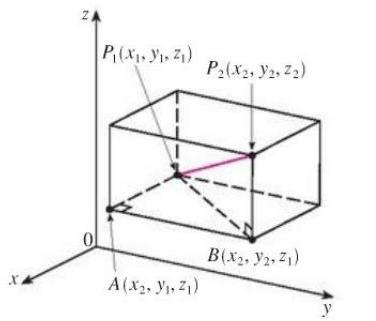
\includegraphics[scale=0.5]{3D-distance.jpg}
\caption{Distances in 3D}
\label{dist}
\end{center}
\end{figure}
\begin{proof}
In Figure \ref{dist}, the pink line represents the distance $|P_1P_2|$, and a rectangular prism is constructed using the two points as opposite vertices. Refer to the figure for points $A,B$ defined above.
\begin{gather*}
    |P_1A| = |x_2-x_1|\hspace{35pt}|AB| = |y_2-y_1|\hspace{35pt}|BP_2| = |z_2-z_1|
\end{gather*}
Using the Pythagorean theorem:
\begin{gather*}
    |P_1P_2|^2 = |P_1B|^2 + |BP_2|^2\\
    |P_1B|^2 = |AB|^2 + |P_1A|^2
\end{gather*}
Now substituting,
\begin{gather*}
    |P_1P_2|^2 = (x_2-x_1)^2+(y_2-y_1)^2+(z_2-z_1)^2\\
    |P_1P_2| = \sqrt{(x_2-x_1)^2+(y_2-y_1)^2+(z_2-z_1)^2}
\end{gather*}
\end{proof}
Applying the distance formula, we can find the equation of a sphere in 3D, since the distance between the center and any point on the sphere is $r$. Squaring both sides of the distance formula with $|P_1P_2| = r$ yields the formula of a sphere with center $C(h,k,l)$.
\begin{gather*}
    (x-h)^2 + (y-k)^2 + (z-l)^2 = r^2
\end{gather*}
\subsection{Vectors}
A \textbf{vector} is any quantity that can be described by a magnitude and a direction. Vectors are often represented by a line that has a direction(indicated with an arrow) and a magnitude(indicated by the length). The notation for vectors here will be: $\vv{AB}$ for a vector with \textbf{initial point} $A$ and \textbf{terminal point} $B$. The magnitude of this vector is $|\vv{AB}|$.

If two vectors $\vv{u}$ and $\vv{v}$ have the same magnitude and direction, they are considered equal. The \textbf{Zero Vector} is a vector with magnitude $0$ and no direction.
\subsubsection{Vector Operations}
If a particle moves along a displacement vector $\vv{AB}$ and another one $\vv{BC}$, then it's total displacement is called the \textbf{sum} of the vectors:
\begin{gather*}
    \vv{AC} = \vv{AB} + \vv{BC}
\end{gather*}
Visually, this \textbf{resultant} vector can be found by positioning the two vectors head to tail and drawing from the first head to the last tail as seen in Fig. \ref{vecadd}.
\begin{figure}[H]
\begin{center}
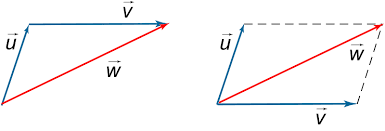
\includegraphics[scale=0.5,angle=2]{vectoraddition.png}
\caption{Vector Addition}
\label{vecadd}
\end{center}
\end{figure}
The resultant $\vv{w}$ can also be obtained by starting both vectors at the same point and drawing the diagonal of the parallelogram indicated in Fig. \ref{vecadd}. Note how the parallelogram can also show that vector addition is commutative.

\textbf{Scalar Multiplication} is multiplying any vector $\vv{v}$ by a constant $c$, forming a new vector $c\vv{v}$. Scalar Multiplication multiplies the magnitude of the vector by $c$. Remember a \textbf{scalar} is a vector with no direction.

The new vector $c\vv{v}$'s magnitude is equal to $c|\vv{v}|$ and it's direction is the same as $\vv{v}$ when $c > 0$ and the opposite when $c < 0$. Notice how $c\vv{v}$ has the same direction as $\vv{v}$ when $c > 0$.

The \textbf{negative} of $\vv{v}$ is $-\vv{v}$, simply $\vv{v}$ in the opposite direction. \textbf{Vector Subtraction} can be defined similar to algebraic subtraction:
\begin{gather*}
    a - b = a + (-b)\\
    \vv{u} - \vv{v} = \vv{u} + (-\vv{v})
\end{gather*}
\begin{figure}[H]
\begin{center}
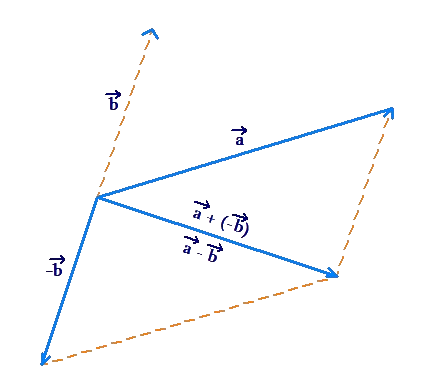
\includegraphics[scale=0.5,angle=0]{vecsub.png}
\caption{Vector Subtraction}
\label{vecsub}
\end{center}
\end{figure}
In Fig \ref{vecsub}, it can be seen how this works. Also, by lining up $\vv{a}$ and $\vv{b}$ at the same starting point, the vector connecting their tails is $\vv{a} - \vv{b}$. Notice how here subtraction is \textit{not} commutative.
\subsubsection{Components and Resultants}
To use vector mathematically, it makes sense to introduce a coordinate system. By convention, the vector starts at the origin and since 2 points define a line, only 2(or 3 in 3D) coordinates are needed to define a vector:
\begin{gather*}
    \vv{v} = \langle a,b \rangle
\end{gather*}
$\langle \rangle$ are used instead of $()$ to show that this is a vector and not a point. This representation from the origin to a particular point makes $\vv{v}$ a \textbf{position vector}.

If the vector doesn't start at the origin, and instead goes between two points $A(x_1,y_1,z_1)$ and $B(x_2,y_2,y_2)$ then:
\begin{gather*}
    \vv{AB} = \vl x_2 - x_1, y_2 - y_1, z_2 - z_1 \vr
\end{gather*}
Remember the magnitude of a vector is the length of its line representation, so using the Pythagorean Theorem in coordinates:
\begin{gather*}
    |\vv{v}| = \sqrt{(v_x)^2 + (v_y)^2}
\end{gather*}
Thinking about the vector addition triangle, to add/subtract two vectors, just add/subtract their components(coordinates). The same works for scalar multiplication, because of similar triangles(scaling up).

Sometimes vectors need to be greater than three dimensions, and so to represent $n$-dimensional vectors, the set $V_n$ represents the set of all possible $n$-dimensional vectors:
\begin{gather*}
    \vv{v_n} = \vl x,y,z...n \vr \in V_n
\end{gather*}
\subsubsection{Vector Properties}
\begin{gather}
    \vv{a} + \vv{b} = \vv{b} + \vv{a}\\
    \vv{a} + 0 = \vv{a}\\
    c(\vv{a} + \vv{b}) = c\vv{a} + c\vv{b}\\
    (\vv{a} + \vv{b}) + \vv{c} = \vv{a} + (\vv{b} + \vv{c})\\
    \vv{a} - \vv{a} = \vv{a} + -\vv{a} = 0\\
    (c+d)\vv{a} = c\vv{a} + c\vv{b}
\end{gather}
These are easily proved, either algebraically or geometrically.
\subsubsection{Unit Vectors}
Consider three 3D vectors:
\begin{gather*}
    \hat{i} = \vl 1,0,0 \vr\hspace{35pt}\hat{j} = \vl 0,1,0 \vr\hspace{35pt}\hat{k} = \vl 0,0,1 \vr
\end{gather*}
These \textbf{unit vectors} all have magnitude $1$ and point in the $x,y,z$ directions. This is interesting because any vector can now be written as scalar multiples of unit vectors:
\begin{gather*}
    \vv{v} = \vl x,y,z \vr = \vl x,0,0 \vr + \vl 0,y,0 \vr + \vl 0,0,z \vr = x\hat{i} + y\hat{j} + z\hat{k}
\end{gather*}
In essence, this notation represents any vector as the vector sum of its components in the $x,y,z...n$ directions.

In general, if $|\vv{v}| \neq 0$, then the unit vector $\hat{u}$ in the $v$-direction is:
\begin{gather*}
    \hat{u} = \dfrac{\vv{v}}{|\vv{v}|}
\end{gather*}
To show why this is true:
\begin{gather*}
    \vv{v} = |\vv{v}|\hat{u}\\
    \hat{u} = \dfrac{\vv{v}}{|\vv{v}|}
\end{gather*}
This is true since $|\vv{v}|$ is a scalar quantity.
\subsection{The Dot Product}
Addition, Subtraction, and Scalar Multiplication are possible, but can you multiply a vector by another vector? One way to do it is called the \textbf{dot product}.

Given $\vv{a} = \vl x_1,y_1,z_1 \vr$ and $\vv{b} = \vl x_2,y_2,z_2 \vr$, the dot product of these is:
\begin{gather*}
    \vv{a} \vdot \vv{b} = x_1x_2 + y_1y_2 + z_1z_2
\end{gather*}
Note that the dot product is \textit{not a vector} but simply a number(scalar). As a result, this product is often called the \textbf{scalar product}.

Some properties of the dot product are similar to numbers:
\begin{gather}
    \vv{a} \vdot \vv{a} = |\vv{a}|^2\\
    \vv{a} \vdot \vv{b} = \vv{b} \vdot \vv{a}\\
    \textrm{\textbf{0}} \vdot \vv{a} = 0
\end{gather}
These can be proved easily by looking at the vector coordinates. They should also make sense. Associative Property also works here(not shown).
\subsubsection{Visualizing the Dot Product}
The dot product of two vectors that start at the same point can be given in terms of the angle $\theta$ between them, where $\theta \in [0,\pi]$. This should make sense, because if $\theta > \pi$ then there would be a smaller angle on the other side(think reflex angles). This new definition is used a lot more in physics(ex. work):
\begin{gather*}
    \vv{a} \vdot \vv{b} = |\vv{a}||\vv{b}|cos(\theta)
\end{gather*}
\begin{proof}
Imagine a triangle $\Delta ABO$ where $OA,OB,AB$ represent $\vv{a},\vv{b},\vv{a}-\vv{b}$ respectively. Applying the law of cosines to $\theta = \measuredangle BOA$:
\begin{gather*}
    |\vv{a} - \vv{b}|^2 = |\vv{a}|^2 + |\vv{b}|^2 - 2|\vv{a}||\vv{b}|cos(\theta)\\
    (\vv{a} - \vv{b})\vdot(\vv{a} - \vv{b}) = \vv{a} \vdot \vv{a} + \vv{b} \vdot \vv{b} - 2|\vv{a}||\vv{b}|cos(\theta)\\
    \vv{a} \vdot \vv{a} - \vv{a} \vdot \vv{b} - \vv{b} \vdot \vv{a} + \vv{b} \vdot \vv{b} = \vv{a} \vdot \vv{a} + \vv{b} \vdot \vv{b} - 2|\vv{a}||\vv{b}|cos(\theta)\\
    -2(\vv{a} \vdot \vv{b}) = -2|\vv{a}||\vv{b}|cos(\theta) \implies \vv{a} \vdot \vv{b} = |\vv{a}||\vv{b}|cos(\theta)
\end{gather*}
\end{proof}
Using this we can conclude:
\begin{gather*}
    cos(\theta) = \dfrac{\vv{a} \vdot \vv{b}}{|\vv{a}||\vv{b}|}
\end{gather*}
Now since $\theta$ is the angle in between $\vv{a}$ and $\vv{b}$, these vectors are \textbf{perpendicular} or \textbf{orthogonal} if the angle between them is $90^{\circ} = \frac{\pi}{2}$ which leads to:
\begin{gather*}
    \vv{a} \vdot \vv{b} = |\vv{a}||\vv{b}|cos\bigg(\dfrac{\pi}{2}\bigg) = 0
\end{gather*}
So two vectors are \textbf{orthogonal} if and only if their dot product $= 0$.
\subsubsection{Direction Angles and Direction Cosines}
The \textbf{direction angles} of any nonzero vector $\vv{v}$ are the specific angles $\alpha,\beta,\gamma \in [0,\pi]$ that $\vv{v}$ makes with the positive $xyz$ axes. The cosines of these angles are called \textbf{direction cosines}.
\begin{gather*}
    cos(\alpha) = \dfrac{\vv{a} \vdot \hat{i}}{|\vv{a}||\hat{i}|} = \dfrac{\vl x_1,y_1,z_1 \vr \vdot \vl 1,0,0 \vr}{|\vv{a}|*1} = \dfrac{x_1}{|\vv{a}|}
\end{gather*}
Similarly:
\begin{gather*}
    cos(\beta) = \dfrac{y_1}{|\vv{a}|}\hspace{45pt}cos(\gamma) = \dfrac{z_1}{|\vv{a}|}
\end{gather*}
By squaring all expressions and using $(x_1)^2 + (y_1)^2 + (z_1)^2 = |a|^2$(dist. formula):
\begin{gather*}
    cos^2(\alpha) + cos^2(\beta) + cos^2(\gamma) = 1
\end{gather*}
Also, because of scalar multiplication:
\begin{gather*}
    \vv{a} = \vl x_1,y_1,z_1 \vr = \vl |\vv{a}|cos(\alpha),|\vv{a}|cos(\beta),|\vv{a}|cos(\gamma) \vr = |\vv{a}|\vl cos(\alpha),cos(\beta),cos(\gamma)\vr\\
    \dfrac{\vv{a}}{|\vv{a}|} = \vl cos(\alpha),cos(\beta),cos(\gamma)\vr = \hat{a}
\end{gather*}
So the vector made up of direction cosines of $\vv{a}$ is the unit vector in the \textbf{a}-direction, which makes sense since $cos(\theta) = 1 * cos(\theta)$, and $|\hat{a}| = 1$
\subsubsection{Projections}
\begin{figure}[H]
\begin{center}
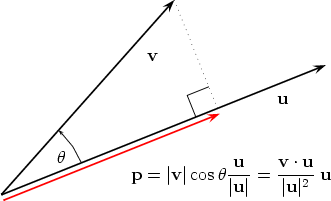
\includegraphics[scale=0.5,angle=0]{vecproj.png}
\caption{Vector Projections}
\label{vecproj}
\end{center}
\end{figure}
The figure above shows a \textbf{vector projection}, which is the vector component of $\vv{v}$ in the $\vv{u}$ direction, and it is represented by $\vv{p}$. It is obtained by first taking a \textbf{scalar projection}, which is the component of $\vv{v}$ along $\vv{u} = |\vv{v}|cos(\theta)$ and multiplying that by $\hat{u} = \frac{\vv{u}}{|\vv{u}|}$, the unit vector in the u-direction.
\begin{gather*}
    comp_a \vv{b} = \dfrac{\vv{a}}{|\vv{a}|}|\vv{b}|*cos(\theta) = \dfrac{\vv{a} \vdot \vv{b}}{|\vv{a}|}\\
    proj_a \vv{b} = \hat{a}*comp_a \vv{b} = \dfrac{\vv{a}}{|\vv{a}|}\bigg[\dfrac{\vv{a} \vdot \vv{b}}{|\vv{a}|}\bigg] = \vv{a}\bigg[\dfrac{\vv{a} \vdot \vv{b}}{|\vv{a}|^2}\bigg]
\end{gather*}
\subsection{The Cross Product}
A second type of vector product is called the \textbf{cross product}. However this time the product is not a scalar but an actual vector, and the cross product is often called the \textbf{vector product}.
\subsubsection{Cross Products and Determinants}
If $\vv{a} = \vl x_1,y_1,z_1 \vr$ and $\vv{b} = \vl x_2, y_2, z_2\vr$, then their cross product $\vv{a} \times \vv{b}$ is:
\begin{gather*}
    \vv{a} \times \vv{b} = \vl y_1z_2 - z_1y_2, z_1x_2 - x_1z_2, x_1y_2 - y_1x_2 \vr
\end{gather*}
This is an interesting product for one because $\vv{a} \times \vv{b}$ will always be $\perp$ to $\vv{a}$ and $\vv{b}$(shown later). Notice that cross products are only defined for 3D vectors $\vv{a}$ and $\vv{b}$.

Cross products are often denoted using \textbf{determinants}, for example an order 2 determinant:
\begin{gather*}
    \begin{vmatrix}
    a & b\\
    c & d
    \end{vmatrix}
    \implies
    \det
    \begin{pmatrix}
    a & b\\
    c & d
    \end{pmatrix}
    = ad - bc
\end{gather*}
Now an order 3 determinant can be defined with order 2 determinants:
\begin{gather*}
\det
    \begin{vmatrix}
    x_1 & x_2 & x_3\\
    y_1 & y_2 & y_3\\
    z_1 & z_2 & z_3
    \end{vmatrix}
    =
    x_1
    \begin{vmatrix}
    y_2 & y_3\\
    z_2 & z_3
    \end{vmatrix}
    - x_2
    \begin{vmatrix}
    y_1 & y_3\\
    z_1 & z_3
    \end{vmatrix}
    + x_3
    \begin{vmatrix}
    y_1 & y_2\\
    z_1 & z_2
    \end{vmatrix}
\end{gather*}
Notice how this works: For every $x_i$ in column $i$, $x_i$ is multiplied by the order 2 determinant found when the $x$-row and column $i$ are both deleted.

Now for cross products, when two vectors $\vv{a} = x_1\hat{i} + x_2\hat{j} + x_3\hat{k}$ and $\vv{b} = y_1\hat{i} + y_2\hat{j} + y_3\hat{k}$, their cross product is shown in this determinant:
\begin{gather*}
    \vv{a} \times \vv{b} =
    \begin{vmatrix}
    x_2 & x_3\\
    y_2 & y_3
    \end{vmatrix}
    \hat{i} -
    \begin{vmatrix}
    x_1 & x_3\\
    y_1 & y_3
    \end{vmatrix}
    \hat{j} +
    \begin{vmatrix}
    x_1 & x_2\\
    y_1 & y_2
    \end{vmatrix}
    \hat{k}
    =
    \begin{vmatrix}
    \hat{i} & \hat{j} & \hat{k}\\
    x_1 & x_2 & x_3\\
    y_1 & y_2 & y_3
    \end{vmatrix}
\end{gather*}
One interesting consequence of the cross product is that $\vv{a} \times \vv{b}$ is orthogonal(perpendicular) to $\vv{a}$ and $\vv{b}$. For this to even be possible for any vectors $\vv{a}$ and $\vv{b}$, this must take place in $V_3$.
\begin{proof}
This is easily proved by showing that $(\vv{a} \times \vv{b}) \vdot \vv{a} = 0$ and also for $\vv{b}$.
\end{proof}
\subsubsection{Visualizing Cross Products}
$\vv{a} \times \vv{b}$ is perpendicular to the plane of $\vv{a}$ and $\vv{b}$, and so it is always perpendicular to both vectors. To find if $\vv{a} \times \vv{b}$ points up or down, use the \textbf{right hand rule} with fingers curling in the direction of rotation from $\vv{a}$ to $\vv{b}$ on the smaller angle($\leqslant 180^{\circ})$.

To find the magnitude of the cross product: Given $\theta$, the angle between $\vv{a}$ and $\vv{b}$(the smaller one):
\begin{gather*}
    |\vv{a} \times \vv{b}| = |\vv{a}||\vv{b}|\sin(\theta)
\end{gather*}
\begin{proof}
Expand the vector coordinates to show that:
\begin{gather*}
    |\vv{a} \times \vv{b}|^2 = |\vv{a}|^2|\vv{b}|^2(1 - \cos^2(\theta)) = |\vv{a}|^2|\vv{b}|^2\sin^2(\theta)
\end{gather*}
\end{proof}
Note in this proof that square root of both sides yields $\sqrt{\sin^2(\theta)} = |\sin(\theta)| = \sin(\theta)$ for all $\theta \in [0,\pi]$.

Using this, two nonzero vectors are parallel if and only if $\vv{a} \times \vv{b} = 0$, because $\vv{a} \times \vv{b} = 0$ when $\theta = 0^{\circ}$ or $180^{\circ}$, which only happens when $\vv{a} \parallel \vv{b}$.
\subsubsection{Interpreting the Cross Product}
One interpretation of the magnitude of the cross product is here:
\begin{figure}[H]
\begin{center}
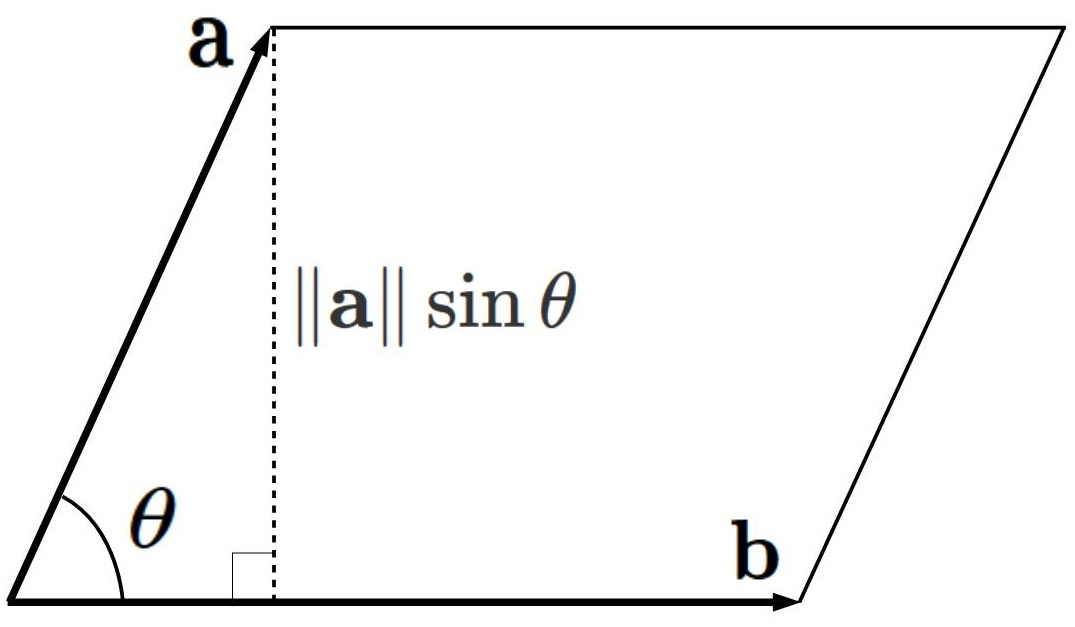
\includegraphics[scale=0.15,angle=0]{crossarea.jpg}
\caption{Area of a Parallelogram}
\label{crossarea}
\end{center}
\end{figure}
In Figure \ref{crossarea}, the area of a parallelogram formed by two vectors $\vv{a}$ and $\vv{b}$ is shown. This area can be expressed as:
\begin{gather*}
    A = Bh = |\vv{b}|*h = |\vv{b}|*(|\vv{a}|\sin(\theta)) = |\vv{a} \times \vv{b}|
\end{gather*}
Notice how the area is $|\vv{a} \times \vv{b}|$ not $\vv{a} \times \vv{b}$. This is because the cross product is a vector, and also in general $\vv{a} \times \vv{b} \neq \vv{b} \times \vv{a}$. These two products will have the same magnitude but will point in opposite directions(right hand rule).

Also, because the cross product is always perpendicular to both vectors:
\begin{gather*}
    \hat{i} \times \hat{j} = \hat{k}\hspace{75pt}\hat{j} \times \hat{i} = -\hat{k}
\end{gather*}
These unit vectors will be perpendicular to each other, also notice how $\hat{k}$ and $-\hat{k}$ point in opposite directions but both have a magnitude of $1$.

Notice how(determinants):
\begin{gather*}
    \vv{a} \vdot (\vv{b} \times \vv{c}) =
    \begin{vmatrix}
    a_1 & a_2 & a_3\\
    b_1 & b_2 & b_3\\
    c_1 & c_2 & c_3
    \end{vmatrix}
\end{gather*}
This combined product is called a \textbf{scalar triple product}, because it combines three vectors into a single scalar. Now why is this important? Refer to the figure below:
\begin{figure}[H]
\begin{center}
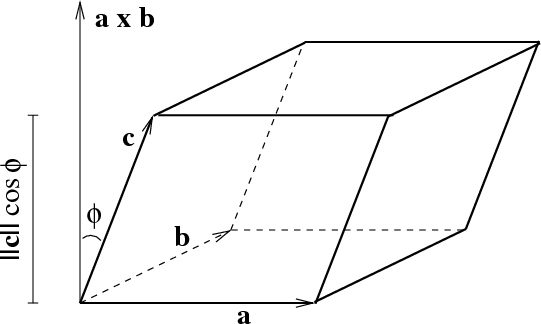
\includegraphics[scale=0.3,angle=0]{crossvol.png}
\caption{Volume of a  Parallelepiped}
\label{crossvol}
\end{center}
\end{figure}
We know from Figure \ref{crossarea} that the base of this figure is a parallelogram with area $|\vv{a} \times \vv{b}|$.
\begin{gather*}
    V = Ah = |\vv{a} \times \vv{b}|h = |\vv{a} \times \vv{b}||\vv{c}|\cos(\phi) = |\vv{c} \vdot (\vv{a} \times \vv{b})|
\end{gather*}
Notice how this is a form of the scalar triple product. Also note that if the volume determined this way is zero, then all three vectors must lie in the same plane, since $\vv{a} \times \vv{b} \perp \vv{c}$.
\subsubsection{Applications}
One application of the cross product is in physics, in torque for example:
\begin{gather*}
    \vv{\tau} = \vv{r} \times \vv{F}
\end{gather*}
This is because the only force that can turn something is the component of it that is perpendicular to the $\vv{r}$. This is also why the direction of a torque can be found using the right hand rule.
\subsection{Equations of Lines and Planes}
Equipped with cross and dot products, we can come up with new definitions in geometry, that are easier to use in 3D space.
\subsubsection{Lines}
A line can be determined in a plane by giving a point and a direction(slope), which is how point-slope form works. Similarly, a 3D line can be defined using a point $P_0(x_0,y_0,z_0)$ and a direction, which here takes the form of a vector $\vv{v}$ parallel to the line. Now draw position vectors $\vv{r_0}$ and $\vv{r}$ to $P_0$ and $P(x,y,z)$ which will represent any point on the line. Now imagine a final vector $\vv{a}$ which goes between $P$ and $P_0$ on the line, and since both \textbf{$r$}-vectors start on the same point:
\begin{gather*}
    \vv{a} = \vv{r} - \vv{r_0}\\
    \vv{r} = \vv{r_0} + \vv{a}
\end{gather*}
Since $\vv{a}$ is on the line, $\vv{a}$ and $\vv{v}$ are parallel, which means $\vv{a} = \vv{v}t$ for some scalar $t$(both vectors point in the same direction but have different lengths).
\begin{gather*}
    \vv{r} = \vv{r_0} + \vv{v}t
\end{gather*}
This is the \textbf{vector equation} of the line. The line is traced out as the \textbf{parameter} $t$ varies. When $t > 0$, $\vv{r}$ traces on one side of $P_0$ and when $t < 0$, $\vv{r}$ traces the other side.

Rewriting $\vv{v} = \vl a,b,c \vr$, then $\vv{v}t = \vl ta, tb, tc\vr$. For our two position vectors $\vv{r} = \vl x,y,z \vr$ and $\vv{r_0} = \vl x_0, y_0, z_0 \vr$ so:
\begin{gather*}
    \vl x,y,z \vr = \vl x_0 + at, t_0 + bt, z_0 + ct \vr
\end{gather*}
Finally, equating components:
\begin{gather*}
    x = x_0 + at\hspace{30pt}y = y_0 + bt\hspace{30pt}z = z_0 + ct
\end{gather*}
These are called \textbf{parametric equations}(can you see why?) and they trace out a line, as each value of $t$ gives a point $(x,y,z)$ on the line. Notice the similarity between this and $y = mx + b$.

Notice how any vector $\vv{v}$ parallel to the line could be used(with any magnitude) and the same line will be formed. If we use $\vv{v} = \vl a,b,c \vr$ then the numbers $a,b,c$ are called the \textbf{direction numbers} of the line. Since any magnitude of $\vv{v}$ could be used, the same line will be formed if $\vv{v} = \vl na, nb, nc \vr$.

We can eliminate the parameter $t$ from all parametric equations by solving for it and substituting:
\begin{gather*}
    \dfrac{x-x_0}{a} = \dfrac{y - y_0}{b} = \dfrac{z - z_0}{c}
\end{gather*}
for $a,b,c \neq 0$. These non-parametric equations are called the \textbf{symmetric equations} of the line. However, as long as at least one of the direction numbers are not zero, this can be used. Ex. if $a = 0$, then $x = x_0 + (0)t$ and:
\begin{gather*}
    x = x_0\hspace{60pt}\dfrac{y-y_0}{b}=\dfrac{z-z_0}{c}
\end{gather*}
This also shows that the line lies on the plane $x = x_0$(in 3D space).

Since $\vv{v} = \vl a,b,c \vr$, and $\vv{v}$ can be the vector drawn between any two points $P(x_0,y_0,z_0)$ and $P_1(x_1,y_1,z_1)$:
\begin{gather*}
    \vv{v} = \vl a,b,c \vr = \vl x_1 - x_0,y_1-y_0,z_1-z_0 \vr\\
    a = x_1 - x_0\hspace{25pt}b = y_1 - y_0\hspace{25pt}c = z_1-z_0\\
    \dfrac{x - x_0}{x_1 - x_0} = \dfrac{y - y_0}{y_1 - y_0} = \dfrac{z - z_0}{z_1 - z_0}
\end{gather*}
This can also be used as an equation of a line. Notice how you can derive the point slope form of a line from this. If you want to define a \textbf{line segment} instead of a whole line, restrict the parameter $t$.

In fact, if you need to find a line segment between two points $P_0$ and $P_1$, find position vectors $\vv{r_0}$ and $\vv{r_1}$ respectively. Since both position vectors have tips on the line and start at the same point, we can choose $\vv{v} = \vv{r_1} - \vv{r_0}$:
\begin{gather*}
    \vv{r} = \vv{r_0} + \vv{v}t = \vv{r_0} + (\vv{r_1}-\vv{r_0})t = \vv{r_0}(1-t) + \vv{r_1}t
\end{gather*}
As $t$ ranges from $0$ to $1$, $\vv{r}$ traces out the correct line segment between $P_0$ and $P_1$.
\subsubsection{Planes}
To define a plane, a single parallel vector is not enough. However, with a orthogonal($\perp$) vector and an initial point(a plane could be defined as all points perpendicular to the vector on the same "level" as the initial point. This vector $\vv{n}$ is called the \textbf{normal vector}. Let $P_0(x_0,y_0,z_0)$ be the initial point and $P(x,y,z)$ be any point on the plane. Define position vectors $\vv{r}$ and $\vv{r_0}$. Since $\vv{r}$ and $\vv{r_0}$ start at the same point, $\vv{r} - \vv{r_0}$ will also be on the plane orthogonal to $\vv{n}$:
\begin{gather*}
    \vv{n} \vdot (\vv{r} - \vv{r_0}) = 0\\
    \vv{n} \vdot \vv{r} = \vv{n} \vdot \vv{r_0}
\end{gather*}
If $\vv{n} = \vl a,b,c \vr$, $\vv{r} = \vl x,y,z \vr$ and $\vv{r_0} = \vl x_0,y_0,z_0 \vr$:
\begin{gather*}
    \vl a,b,c \vr \vdot \vl x-x_0,y-y_0,z-z_0 \vr = 0\\
    a(x-x_0) + b(y-y_0) + c(z-z_0) = 0
\end{gather*}
This is the \textbf{scalar equation} of a plane. Notice that if $a,b,c$ are not all $0$ then the equation of a plane can take the form:
\begin{gather*}
    ax + by + cz + d = 0
\end{gather*}
The great thing about normal vectors is that they act as "markers" for planes. For example, two planes with normals $\vv{n_1}$ and $\vv{n_2}$ are parallel if their vectors are parallel, in other words is $\vv{n_2} = c\vv{n_1}$, where $c$ is a constant. If they aren't parallel, then they intersect in a line and the angle between the two planes($< 90^{\circ}$ is the angle between their vectors(use dot product).

Since the intersection of two planes is a line, a line can be written as the intersection of two planes.
\begin{gather*}
    \dfrac{x-x_0}{a} = \dfrac{y-y_0}{b}\hspace{45pt}\dfrac{y-y_0}{b} = \dfrac{z-z_0}{c}
\end{gather*}
These two equations are equations of planes, and when set equal become an equation of a line!

Lastly, the distance between two \textit{parallel} planes is:
\begin{gather*}
    D = \dfrac{|ax_1 + by_1 + cz_1 + d|}{\sqrt{a^2 + b^2 + c^2}}
\end{gather*}
This can be found by finding the projection of a vector between one point on each plane on their \textit{shared} normal vector.
\subsection{Cylinders and Quadric Surfaces}
Planes are a more simple type of surface, and graphing those are not too difficult. However, in more complex surfaces it is often useful to get the cross sections of the surface on different planes, which are called \textbf{traces}.
\subsubsection{Cylinders}
A cylinder is a type of surface that is made up of a set of lines(called \textbf{rulings}) that are all parallel to a given(central) line and pass through a curved plane. Note that a cylinder does not always have to be the cylinder you're thinking of(see \textbf{parabolic cylinder}).
\subsubsection{Quadric Surfaces}
A \textbf{quadric surface} is the result of a degree 2 polynomial equation written in $x,y,z$:
\begin{gather*}
    ax^2 + by^2 + cz^2 + dxy + eyz + fxz + gx + hy + Iz + j = 0
\end{gather*}
Quadric surfaces are the 3D equivalent to the 2D conics(see 11.5)
\subsubsection{Sketching Surfaces}
The main method for sketching surfaces is to use traces(cross-sections) that are parallel to the $xyz$ planes. For example, to graph:
\begin{gather*}
    \dfrac{x^2}{a^2} + \dfrac{y^2}{b^2} + \dfrac{z^2}{c^2} = 1
\end{gather*}
First find the traces in each direction, by substituting $x=k$ then $y=k$ and finally $z=k$, where $k$ is any number. This simplifies the 3D surface into a bunch of slices of 2D curves.
\begin{gather*}
    \dfrac{x^2}{a^2} + \dfrac{y^2}{b^2} = 1 - \dfrac{k^2}{c^2}
\end{gather*}
This is an example of $z = k$, where every term on the right side is a constant, which means that when $k^2 < c^2$ then the right side is $< 1$ and the trace is an ellipse.
\subsection{Cylindrical and Spherical Coordinates}
In 3D, polar coordinates are expressed in two different but useful coordinate systems.
\subsubsection{Cylindrical Coordinates}
In \textbf{cylindrical coordinates} any point in 3D space can be represented by three numbers $(r,\theta,z)$ where $r$ and $\theta$ are the polar coordinates of the point on 2D space(on the $xy$ plane), and $z$ is the $z$-coordinate of the point.
\begin{figure}[H]
\begin{center}
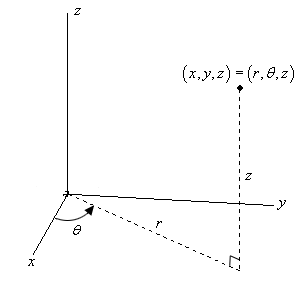
\includegraphics[scale=0.6,angle=0]{cylcoords.png}
\caption{Cylindrical Coordinates}
\label{cylcoords}
\end{center}
\end{figure}
To convert from cylindrical to rectangular:
\begin{gather*}
    x = r\cos(\theta)\hspace{20pt}y=r\sin(\theta)\hspace{20pt}z=z
\end{gather*}
To convert back to rectangular:
\begin{gather*}
    r^2 = x^2 + y^2\hspace{20pt}\tan(\theta) = \dfrac{y}{x}\hspace{20pt}z=z
\end{gather*}
Cylindrical coordinates are the best to choose when dealing with symmetry about a certain axis(especially the $z$-axis). Imagine a cylinder around the $z$-axis $x^2 + y^2 = c^2$. In cylindrical coordinates, that equation is $r=c$, since $\theta$ and $z$ can vary to create the cylinder.
\subsubsection{Spherical Coordinates}
\begin{figure}[H]
\begin{center}
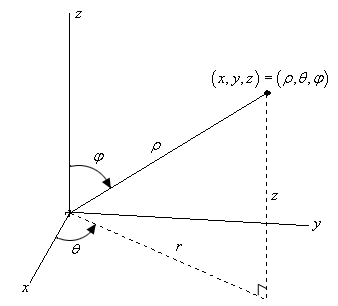
\includegraphics[scale=0.6,angle=0]{spherical.png}
\caption{Spherical Coordinates}
\label{sphcoords}
\end{center}
\end{figure}
The \textbf{spherical coordinates} of a point in 3D can be described using $(\rho, \theta, \phi)$, where $\rho = |OP|$(dist. from origin to $P$) and $\theta$ is the same angle in cylindrical. $\phi$ is the angle between $\rho$ and the $z$-axis.
\begin{gather*}
    \rho \geqslant 0\hspace{25pt}0 \leqslant \phi \leqslant \pi
\end{gather*}
This coordinate system is useful when dealing with symmetry about a point. Easiest way to see this is with a sphere, with equation $\rho = c$, since $\theta$ and $\phi$ can vary wildly, drawing out a sphere with all points a distance $\rho = c$ away from the origin.

Some common spherical coordinate uses are $\theta = c$(a half plane), $\phi = c$, a cone above the $xy$ plane when $c \in [0, \frac{\pi}{2}]$ and below when $c \in [\frac{\pi}{2},\pi]$.

To convert from spherical to rectangular, refer to Figure \ref{sphcoords}, and imagine points $P(x,y,z)$, $Q$, which is when a line is drawn straight from $P$ to the $z$-axis, and $P'$, which is when a line is drawn straight down from $P$ to the $xy$ plane. Using the Alt. Interior Angle theorem, the angle between $\rho$ and $z$ in the figure is $\phi$:
\begin{gather*}
    z = \rho\cos(\phi)\hspace{20pt}x = r\cos(\theta) = \rho\sin(\phi)\cos(\theta)\hspace{20pt}y = r\sin(\theta) = \rho\sin(\phi)\sin(\theta)
\end{gather*}
Finally, to convert from rectangular to spherical, use the distance formula(along with the above):
\begin{gather*}
    \rho^2 = x^2 + y^2 + z^2
\end{gather*}
\section{Vector Functions}
\subsection{Vector Functions and Space Curves}
\subsubsection{Limits and Continuity}
Since a function in a basic sense is a mapping of one element of the \textbf{domain} to another element in the \textbf{range}, a \textbf{vector-valued function} is a mapping from a scalar domain to a vector range. In simple terms, every number $t$ in the domain can be mapped to some vector in $V_3$ defined as $\vv{r} = \ve{f(t),g(t),h(t)}$, where $f,g$ and $h$ are the \textbf{component functions} of $\vv{r}$:
\begin{gather*}
    \vv{r}(t) = \ve{f(t),g(t),h(t)} = f(t)\hat{i} + g(t)\hat{j} + h(t)\hat{k}
\end{gather*}
As usual, the domain of $\vv{r}(t)$ is the set of all $t$ where $f,g$ and $h$ are defined. The \textbf{limit} of a vector function is simply the limit of it's components:
\begin{gather*}
    \lim_{t \to c} \vv{r}(t) = \ve{\lim_{t \to c} f(t), \lim_{t \to c} g(t), \lim_{t \to c} h(t)}
\end{gather*}
If all limits exist, then the vector function's limit exists. If the limit of $\vv{r}(t)$ is $\vv{L}$, then the magnitude and direction of $\vv{r}(t)$ approaches that of $\vv{L}$ for values close to $c$. Limits of vector functions obey the same laws as real functions do. It follows that:

Any vector function $\vv{r}(t)$ is continuous at $c$ if:
\begin{gather*}
    \lim_{t \to c} \vv{r}(t) = \vv{r}(c)
\end{gather*}
It follows that $\vv{r}(t)$ is continuous if and only if it's components are.
\subsubsection{Space Curves}
Imagine a vector function $\vv{r}$ with components $f,g$ and $h$, which are all continuous. Now imagine a curve C drawn using the set of points:
\begin{gather*}
    x = f(t)\hspace{40pt}y=g(t)\hspace{40pt}z=h(t)
\end{gather*}
Look familiar? Yes, these are \textbf{parametric equations} of the curve C, and the vector $\vv{r}$ traces out C as $t$ varies. These are just like 3D parametric equations! If C fits the case, the C is a \textbf{space curve}.
\subsubsection{Visualizing Space Curves}
Computer drawing with space curves is a good way to visualize it, but when you do not have technology at your disposal it's good to have a way of visualizing these. You can think of the parametric equations as "traces", similar to drawing surfaces.

Another way to visualize space curves is to draw them on surfaces, for example you could visualize a curve of intersection between two cylinders.
\subsection{Derivatives and Integrals of Vector Functions}
\subsubsection{Derivatives}
Because the limit of a vector function is defined similar to a normal function, we can define the derivative similarly as well(since derivatives are based off limits).

The \textbf{derivative} $\vv{r}'$ of a vector function $\vv{r}$:
\begin{gather*}
    \dfrac{d\vv{r}}{dt}=\vv{r}'(t) = \lim_{h \to 0}\dfrac{\vv{r}(t+h) - \vv{r}(t)}{h}
\end{gather*}
Remember that $\vv{r}(t+h)$ and $\vv{r}(t)$ are both position vectors that start at the same point. So $\vv{r}(t+h) - \vv{r}(t)$ is the distance between them because of simple vector subtraction, which can be treated as secant vector on the curve. As $h \to 0$, the secant vector becomes a \textbf{tangent vector} as long as $\vv{r}'(t)$ exists and $\vv{r}'(t) \neq 0$. So now the \textbf{tangent line} is defined as the line parallel to the vector $\vv{v} = \vv{r}'(t)$ that goes through the point of tangency $P$.

The \textbf{unit tangent vector}, or the unit vector in the direction of the tangent:
\begin{gather*}
    \vv{T}(t) = \dfrac{\vv{r}'(t)}{|\vv{r}'(t)|}
\end{gather*}
However, there is an easier way to get the derivative of a vector function. If $\vv{r} = \ve{f(t),g(t),h(t)}$, where $f,g$ and $h$ are differentiable:
\begin{gather*}
    \vv{r}'(t) = \ve{f'(t),g'(t),h'(t)}
\end{gather*}
This is easily shown by applying the limit definition to each component.

The \textbf{second derivative} is simply the derivative of the derivative, or $\vv{r}''(t)$.

A curve of a function $\vv{r}(t)$ is smooth on an interval if $\vv{r}'$ is continuous and $\vv{r}'(t) \neq 0$, except possibly on the endpoints.

Differentiation rules are the same for a vector function as for a normal function. Dot products and cross products of vectors obey the product rule.
\subsubsection{Integrals}
We can apply the same vector derivative logic to integration with limits to Riemann sums:
\begin{gather*}
    \int_a^b \vv{r}(t) dt = \lim_{n \to \infty} \sum_{i = 1}^n \vv{r}(t_i)\Delta t
\end{gather*}
Applying this to each component, we get:
\begin{gather*}
    \int_a^b \vv{r}(t) dt = \Bigg\vl\bigg[\int_a^b f(t) dt\bigg], \bigg[\int_a^b g(t) dt\bigg], \bigg[\int_a^b h(t) dt\bigg]\Bigg\vr
\end{gather*}
The FTC also works with vector functions:
\begin{gather*}
    \int_a^b \vv{r}(t) dt = \bigg[\vv{R}(t)\bigg]_a^b = \vv{R}(b) - \vv{R}(a)
\end{gather*}
where $\vv{R}$ is the antiderivative of $\vv{r}$.
\subsection{Arc Length and Curvature}
\subsubsection{Arc Length}
From chapter 11, the arc length of a 2D curve with parametric equations $x = f(t)$ and $y = g(t)$ between $a$ and $b$ has arc length:
\begin{gather*}
    L = \int_a^b \sqrt{\bigg[f'(t)\bigg]^2 + \bigg[g'(t)\bigg]^2}\d t
\end{gather*}
where $f'$ and $g'$ must be continuous on the interval. This is found by taking the limit of an n-sided inscribed polygon(as $n \to \infty$). Doing the exact same thing with parametric equations $x = f(t), y = g(t), z = h(t)$. If the curve is traced exactly one time from $a$ to $b$:
\begin{gather*}
    L = \int_a^b \sqrt{\bigg[f'(t)\bigg]^2 + \bigg[g'(t)\bigg]^2+\bigg[h'(t)\bigg]^2}\d t\\
    = \int_a^b \sqrt{\bigg[\dfrac{dx}{dt}\bigg]^2 + \bigg[\dfrac{dy}{dt}\bigg]^2+\bigg[\dfrac{dz}{dt}\bigg]^2}\d t\\
    = \int_a^b |\vv{r}'(t)|\d t
\end{gather*}
Even though different \textbf{parametrizations} of a curve C are possible(different parametric equations that show the same curve), the arc length found will be the same.

Let C be a curve given by $\vv{r}(t) = f(t)\hat{i} + g(t)\hat{j} + h(t)\hat{k}$ for $t \in [a,b]$, and C is traced exactly once in the interval. C's \textbf{arc length function}:
\begin{gather*}
    s(t) = \int_a^t |\vv{r}'(u)| \d u = \int_a^t \sqrt{\bigg[\dfrac{dx}{du}\bigg]^2 + \bigg[\dfrac{dy}{du}\bigg]^2+\bigg[\dfrac{dz}{du}\bigg]^2}\d u
\end{gather*}
Taking the derivative of both sides and using FTC:
\begin{gather*}
    \dfrac{ds}{dt} = |\vv{r}'(t)|
\end{gather*}
It is often useful to parametrize a curve \textbf{with respect to arc length} because arc length is a distance, which is not relative(doesn't change depending on your coordinate system). If any curve $\vv{r}(t)$ and $s(t)$, the arc length function is given, then you can solve for $t$ asa fucntion of $s$: $t = t(s)$. Now since $\vv{r} = \vv{r}(t) \implies \vv{r} = \vv{r}(t) = \vv{r}(t(s))$. For example, $\vv{r}(t(3))$ represents the position vector of $\vv{r}$ at the point 3 units of arc length from the starting point.
\subsubsection{Curvature}
If C is a smooth curve defined by $\vv{r}(t)$, then $\vv{r}'(t) \neq 0$, also the unit tangent vector $\vv{T}$, which is the unit of the derivative:
\begin{gather*}
    \vv{T}(t) = \dfrac{\vv{r}'(t)}{|\vv{r}'(t)|}
\end{gather*}
Imagining a curve, the direction of $\vv{T}$ will change fast when the curve is sharply curved, and slower when the curve is straighter. The \textbf{curvature} of C at a point is how fast the curve changes direction at that point. It is the rate of change of the unit tangent with respect to arc length. Arc length is used because as mentioned it doesn't change when parameterized:
\begin{gather*}
    \kappa(t) = |\dfrac{d\vv{T}}{ds}|
\end{gather*}
Using the chain rule:
\begin{gather*}
    \dfrac{d\vv{T}}{dt} = \dfrac{d\vv{T}}{ds}\dfrac{ds}{dt}\\
    \kappa = |\dfrac{d\vv{T}}{ds}| = |\dfrac{\frac{d\vv{T}}{dt}}{\frac{ds}{dt}}| = \dfrac{|\vv{T}'(t)|}{|\vv{r}'(t)|}
\end{gather*}
This can be used to show that small circles have large curvature and large circles have smaller curvature. The curvature of a circle with radius $a$ is:
\begin{gather*}
    \kappa = \dfrac{1}{a}
\end{gather*}
The following is often more convenient to use:
\begin{gather*}
    \kappa(t) = \dfrac{|\vv{r}'(t) \times \vv{r}''(t)|}{|\vv{r}'(t)|^3}
\end{gather*}
\begin{proof}
Since $\vv{T} = \dfrac{\vv{r}'}{|\vv{r}'|}$ and $|\vv{r}'| = \dfrac{ds}{dt}$:
\begin{gather*}
    \vv{r}' = |\vv{r}'|\vv{T} = \dfrac{ds}{dt}\vv{T}\\
\end{gather*}
Taking a derivative(use product rule):
\begin{gather*}
    \vv{r}'' = \dfrac{d^2s}{dt^2}\vv{T} + \dfrac{ds}{dt}\vv{T}'
\end{gather*}
Cross both sides, and use the fact that $\vv{T} \times \vv{T} = 0$:
\begin{gather*}
    \vv{r}' \times \vv{r}'' = \bigg(\dfrac{ds}{dt}\bigg)^2(\vv{T} \times \vv{T}')
\end{gather*}
Since $\vv{T}$ is a unit vector, $|\vv{T}(t)| = 1$. Since $1$ is a constant, $\vv{T}$ is orthogonal to $\vv{T}'$. Also using $|\vv{a} \times \vv{b}| = |\vv{a}||\vv{b}| \sin(\theta)$:
\begin{gather*}
    |\vv{r}' \times \vv{r}''| = \bigg(\dfrac{ds}{dt}\bigg)^2|\vv{T} \times \vv{T}'| = \bigg(\dfrac{ds}{dt}\bigg)^2|\vv{T}||\vv{T}'| = \bigg(\dfrac{ds}{dt}\bigg)^2|\vv{T}'|\\
    |\vv{T}'| = \dfrac{|\vv{r}' \times \vv{r}''|}{(ds/dt)^2} = \dfrac{|\vv{r}' \times \vv{r}''|}{|\vv{r}'|^2}\\
    \kappa = \dfrac{|\vv{T}'|}{|\vv{r}'|} = \dfrac{|\vv{r}' \times \vv{r}''|}{|\vv{r}'|^3}
\end{gather*}
\end{proof}
For the special case of a 2D curve with equation $y = f(x)$, we can use $x$ as the parameter: $\vv{r}(x) = x\hat{i} + f(x)\hat{j}\implies\vv{r}''(x) = f''(x)\hat{j}$. When crossing, since $\hat{i} \times \hat{j} = \hat{k}$, and $\hat{j} \times \hat{j} = 0: \vv{r}' \times \vv{r}'' = f''(x)\hat{k}$. Also noting that the arc length in 2D:
\begin{gather*}
    L = |\vv{r}'(x)| = \sqrt{1 + [f'(x)]^2}\\
    \kappa(x) = \dfrac{|f''(x)|}{[1 + (f'(x))^2]^\frac{3}{2}}
\end{gather*}
\subsubsection{Normal and Binormal Vectors}
At any point on a space curve $\vv{r}(t)$, there will be many vectors orthogonal to $\vv{T}$, but you can find one by noting that $|\vv{T}| = 1$, so $\vv{T'} \perp \vv{T}$. NOTE: \textbf{$\vv{T}'$ is not a unit vector!} But if $\vv{r}'$ is smooth(derivative not zero), the \textbf{unit normal vector} $\vv{N}(t)$, the unit vector of the unit tangent's derivative(a mouthful!):
\begin{gather*}
    \vv{N}(t) = \dfrac{\vv{T}'(t)}{|\vv{T}'(t)|}
\end{gather*}
The vector given by $\vv{B}(t) = \vv{T}(t) \times \vv{N}(t)$ is called the \textbf{binormal vector}. Since it's a cross, it is perpendicular to both $\vv{T}$ and $\vv{N}$.
\begin{figure}[H]
\begin{center}
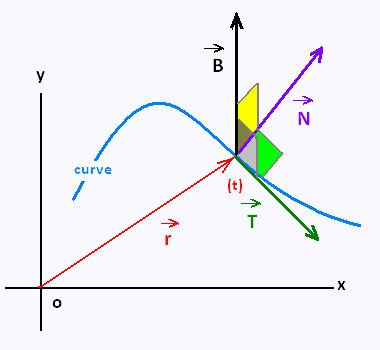
\includegraphics[scale=0.5,angle=0]{tnb.png}
\caption{Tangent, Normal, and Binormal}
\label{tnb}
\end{center}
\end{figure}
The plane defined by $\vv{N}$ and $\vv{B}$ at any point $P$ is called the \textbf{normal plane} at $P$. It contains all lines that are orthogonal to $\vv{T}$. The plane using $\vv{T}$ and $\vv{N}$ is the \textbf{osculating plane} at $P$(\textit{osculum} in Latin means \textit{kiss}). This plane is the closest to containing the part of the curve near $P$. In a 2D curve, this plane is simply the entire plane containing the curve.

The circle that lies in the osculating plane and has the same tangent at $P$, which also lies on the concave side of $C$(the direction $\vv{N}$ points), and has radius $r = \frac{1}{\kappa}$ is the \textbf{osculating circle} at $P$. It best describes how C behaves near $P$, since it shares the same tangent, normal, and curvature.
\subsection{Motion in Space: Velocity and Acceleration}
\end{document}
